
%% LyX 2.1.2dev created this file.  For more info, see http://www.lyx.org/.
%% Do not edit unless you really know what you are doing.
\documentclass[12pt,a4paper,polish,thesis]{dcsbook}
\usepackage[T1]{fontenc}
\usepackage[utf8]{inputenc}
\setcounter{secnumdepth}{3}
\usepackage{babel}
\usepackage{rotfloat}
\usepackage{pdfpages}
\usepackage{amsthm}
\usepackage{graphicx}
\usepackage[unicode=true,pdfusetitle,
 bookmarks=true,bookmarksnumbered=true,bookmarksopen=true,bookmarksopenlevel=1,
 breaklinks=true,pdfborder={0 0 0},backref=false,colorlinks=false]
 {hyperref}
\hypersetup{
 urlcolor=linkcolor,linkcolor=linkcolor,citecolor=linkcolor}

\makeatletter

%%%%%%%%%%%%%%%%%%%%%%%%%%%%%% LyX specific LaTeX commands.
\pdfpageheight\paperheight
\pdfpagewidth\paperwidth

%% Because html converters don't know tabularnewline
\providecommand{\tabularnewline}{\\}
%% A simple dot to overcome graphicx limitations
\newcommand{\lyxdot}{.}


%%%%%%%%%%%%%%%%%%%%%%%%%%%%%% Textclass specific LaTeX commands.
\RequirePackage{dcslib}[2012/01/30]
  \theoremstyle{definition}
  \newtheorem{defn}{\protect\definitionname}[section]

%%%%%%%%%%%%%%%%%%%%%%%%%%%%%% User specified LaTeX commands.
%
%  $Id: thesis-template.lyx,v 1.7 2011/12/22 12:10:18 sobaniec Exp $
%
\AtBeginDocument{% 
        \renewcommand{\tablename}{Tabela}% 
}
\definecolor{tomato}{RGB}{139, 54, 38}
\definecolor{darkblue}{RGB}{36, 92, 165}
\definecolor{darkgreen}{RGB}{0, 127, 14}
\definecolor{bluekeywords}{rgb}{0.13,0.13,1}
\definecolor{greencomments}{rgb}{0,0.5,0}
\definecolor{redstrings}{rgb}{0.9,0,0}

\lstdefinelanguage{XML}
{
  morestring=[s]{>}{<},
  stringstyle=\color{tomato},
  identifierstyle=\color{black},
  keywordstyle=\bfseries\color{darkblue},
  morekeywords={type, Initialize, methodHandle, Execute, eId, parameters, callbackUri, Address, Binding, ExecuteCallback, eid, ExecuteResult, executeResult, ElapsedTime, Error, ExecutorState, Result, Register, Unregister}
}

\lstdefinelanguage{Assembler}
{
  keywordstyle=\bfseries\color{darkblue},
  morekeywords={b__0, Int32, Int64, DistributedPI, Program, Bluepath}
}

\lstset{language=[Sharp]C,
  morecomment=[l]{//}, %use comment-line-style!
morecomment=[s]{/*}{*/}, %for multiline comments
showstringspaces=false,
morekeywords={ abstract, event, new, struct, as, explicit, null, switch, base, extern, object, this, bool, false, string, operator, throw, break, finally, out, true, byte, fixed, override, try, case, float, params, typeof, catch, for, private, uint, char, foreach, protected, ulong, checked, goto, public, unchecked, class, if, readonly, unsafe, const, implicit, ref, ushort, continue, in, return, using, decimal, int, sbyte, virtual, default, interface, sealed, volatile, delegate, internal, short, void, do, is, sizeof, while, double, lock, stackalloc, else, long, static, enum, namespace },
keywordstyle=\color{darkblue},
identifierstyle=\color{black},
emph=[1]{ IRemoteExecutorService, Guid, ServiceUri, RemoteExecutorServiceResult, PerformanceStatistics, ServiceContract, OperationContract, Task, Dictionary, ICoordinatorService, Uri, MapReduceResult, Tuple, DataContract, DataMember, IEnumerable, KeyValuePair, List, IBluepathCommunicationFramework, IExtendedStorage, DistributedCounter, RoundRobinLocalScheduler, DistributedThread },
emph=[2]{ var, from, select, using },
emphstyle=[1]\color{darkgreen},
emphstyle=[2]\color{darkblue}
}

\makeatother

\usepackage{listings}
  \providecommand{\definitionname}{Definicja}
\renewcommand{\lstlistingname}{Listing}

\begin{document}

\author{Piotr~Bazydło\and Zachariusz~Karwacki}


\title{Bluepath -- biblioteka wspomagająca tworzenie programów rozproszonych}


\date{Poznań, 2014}


\supervisor{dr inż. Jacek Kobusiński}

\maketitle



\includepdf{external/karta}


\includepdf[pages=-]{external/bluepath}

\frontmatter

\tableofcontents{}

\begin{abstract}
\dcsstrong{Bluepath -- library supporting creating distributed applications}

The aim of this work is to design a library, which, without complicated
configuration or installation of multiple components, will allow programmers
to implement distributed applications in easy way. A programmer, while
writing an application using a parallel programming model based on
threads, should be able to utilise the computing power of multiple
machines in a cluster. The threads created by the programmer instead
of being executed on one of machine's cores will be executed on one
of the remote machines.

At the time of writing there wasn't available any popular, actively
developed and commercially supported environment for creating distributed
applications in .NET Framework. This kind of enviroment would allow
programmers not only to avoid the need of solving many problems found
in distributed programming by themselves but also to save time. One
of the main goals was to make the library as modular as possible --
this way Bluepath wouldn't strongly depend on the implementation of
its components.

\end{abstract}

\mainmatter


\chapter{Wstęp}
\begin{quote}
\dcsemph{Programming is intrinsically very difficult.}

\begin{flushright}
--- E. Dijkstra
\par\end{flushright}
\end{quote}
Tworzenie aplikacji działających w klastrze jest złożone i wiąże się
z nim wiele problemów takich jak wykrycie zakończenia czy dystrybucja
danych pomiędzy maszynami. Dużo prostsze jest tworzenie aplikacji
wykorzystujących wiele procesorów i rdzeni pojedynczej maszyny. W
niniejszej pracy zaproponowano rozwiązanie czerpiące z obu podejść,
pozwalające zastosować mechanizmy znane z programowania równoległego
przy tworzeniu aplikacji rozproszonych.

W tym rozdziale przedstawione zostaną założony cel oraz zakres pracy,
jej struktura, motywacja oraz podział prac pomiędzy autorów.


\section{Cel i zakres pracy}

\label{sec:intro-cel-i-zakres}Celem pracy było zaprojektowanie biblioteki,
która, bez skomplikowanej konfiguracji czy instalowania wielu składników,
pozwoli jej użytkownikom, programistom, w prosty sposób zaimplementować
program przetwarzający dane w sposób rozproszony. Programista pisząc
program w sposób podobny do tego w jaki pisałby program równoległy,
powinien uzyskać program wykorzystujący moc obliczeniową wielu węzłów
w klastrze. W takim przypadku wątki, zamiast wykonywać się na wielu
rdzeniach jednego procesora, mogą wykonywać się na zdalnych maszynach.


\section{Struktura pracy}

W niniejszej pracy omówiono koncepcję oraz implementację biblioteki
o kodowej nazwie Bluepath. Bieżący rozdział opisuje w dalszej części
motywacje oraz wkład członków zespołu. Rozdział drugi stanowi wstęp
teoretyczny obejmujący definicje oraz przegląd istniejących rozwiązań
-- środowisk przetwarzania rozproszonego. W~rozdziale trzecim została
szczegółowo przedstawiona koncepcja i projekt systemu, a~rozdział
czwarty opisuje implementacje poszczególnych komponentów. Przykładowe
zastosowania biblioteki przy implementowaniu aplikacji obliczeniowych
przedstawia rozdział piąty, a wyniki testów jakościowych, wydajnościowych
i ich analizę -- rozdział szósty. W rodziale siódmym podsumowano przebieg
realizacji, opisano napotkane problemy a także zaproponowano obszary,
w których możnaby kontynuować prace nad usprawnieniem biblioteki.


\section{Motywacja}

W czasie, kiedy rozpoczynano pracę nie było dostępne popularne, aktywnie
rozwijane i wspierane komercyjnie środowisko do przetwarzania rozproszonego
dla .NET Framework (por. punkt \ref{sec:background-Istniej=000105ce-rozwi=000105zania}).
Tego typu środowisko pozwoliłoby użytkownikom uniknąć konieczności
samodzielnego rozwiązywania wielu problemów przetwarzania rozproszonego
oraz zaoszczędzić czas poprzez wykorzystanie dostarczonych mechanizmów.


\section{Udział w pracy poszczególnych członków zespołu}

Niniejsza praca została stworzona przez dwie osoby. Podział prac został
przedstawiony poniżej.


\paragraph{Piotr Bazydło}
\begin{itemize}
\item koncepcja rozwiązania,
\item przegląd i analiza mechanizmów pamięci współdzielonej,
\item przykładowe aplikacje -- DLINQ, system uzupełniania wyrazów,
\item implementacja części testów jakościowych i wydajnościowych,
\item przygotowanie środowiska do przeprowadzenia testów wydajnościowych,
\item implementacja zamków rozproszonych,
\item implementacja planisty szeregującego zadania w oparciu o obciążenie
węzłów,
\item implementacja planisty szeregującego zadania wykorzystującego algorytm
cykliczny,
\item implementacja pamięci rozproszonej na bazie istniejącego rozwiązania,
\item implementacja rozproszonych struktur danych i obiektów.
\end{itemize}

\paragraph{Zachariusz Karwacki}
\begin{itemize}
\item przegląd istniejących rozwiązań,
\item koncepcja rozwiązania,
\item implementacja logiki wątku rozproszonego,
\item implementacja zdalnego wykonawcy,
\item implementacja lokalnego wykonawcy,
\item implementacja mechanizmów logowania zdarzeń,
\item implementacja usługi odnajdywania węzłów,
\item implementacja zarządcy połączeń,
\item implementacja interfejsu do komunikacji z systemem,
\item implementacja części testów jakościowych i wydajnościowych,
\item przykładowe aplikacje -- MapReduce, obliczanie liczby PI,
\item stworzenie skryptów dystrybuujących aplikację w klastrze.\end{itemize}



\chapter{Podstawy teorytyczne}

W tym rozdziale przedstawione zostaną terminy wykorzystywane w dalszej
części pracy oraz zestawienie rozwiązań podobnych tematyką do tej
pracy.


\section{Przetwarzanie równoległe}

\label{sec:background-rownolegle}Jednym z modeli przetwarzania danych
jest przetwarzanie równoległe. Polega ono na przetwarzaniu zbioru
danych jednocześnie na wielu procesorach i rdzeniach. W ten sposób
fragmenty przetwarzania, które nie są od siebie zależne mogą zostać
wykonane w tym samym czasie -- pozwala to skrócić czas przetwarzania.

Jednym ze sposobów prowadzenia przetwarzania równoległego jest wykorzystanie
wątków. Wątki, czasami nazywane lekkimi procesami, wykonują kod niezależnie
od siebie, ale działają we wspólnej przestrzeni adresowej, co pozwala
współdzielić dane, ale wymaga zastosowania mechanizmów synchronizacji.
Podstawowym mechanizmem synchronizacji są zamki. Służą one do realizacji
sekcji krytycznych -- fragmentów kodu, które mogą być wykonywane w
danym momenie tylko przez jeden wątek. 


\section{Przetwarzanie rozproszone}

\label{sec:background-Przetwarzanie-rozproszone} Przetwarzanie rozproszone~\cite{ArpaciDusseau14-Book}
jest szeroko stosowanym podejściem w przypadku przetwarzania dużej
ilości danych, konieczności obsługi wielu zleceń użytkowników w jednostce
czasu czy zapewnienia niezawodności systemu. Problemy, z jakimi zmagają
się programiści aplikacji rozproszonych dotyczą m. in. obsługi awarii
(wraz z rosnącą liczbą elementów systemu rośnie prawdopodobieństwo
awarii jednego z~nich), bezpieczeństwa (zapewnienia poufności, integralności
i autentyczności komunikatów) i komunikacji. Trzeba brać pod uwagę
możliwość utraty pakietu, niedostarczenia potwierdzenia odbioru, maksymalizować
wydajność i przepustowość poprzez minimalizowanie liczby komunikatów
i opóźnień komunikacyjnych. Wykorzystywane w praktyce protokoły sieciowe
rozwiązują także wiele innych problemów, jak np.~zatory w sieci czy
zaległe żądania (ang.~\dcsemph{outstanding requests}). W celu przyspieszenia
tworzenia systemów rozproszonych zaproponowano wprowadzenie abstrakcji
realizujących niezawodną komunikację sieciową i wymianę danych bez
bezpośredniego udziału programisty. 


\subsection{DSM}

\label{sub:background-DSM}Model rozproszonej pamięci współdzielonej
(ang.~\dcsemph{distributed shared memory}, DSM)~\cite{DSM} implementowany
jest na poziomie systemu operacyjnego. Zakłada on udostępnienie wspólnej
przestrzeni adresowej dla wszystkich komputerów biorących udział w
przetwarzaniu. Aplikacje odwołują się do pamięci w tradycyjny sposób.
W przypadku wystąpienia błędu braku strony system operacyjny zajmuje
się sprowadzeniem jej do lokalnej pamięci. Mechanizm DSM nie jest
obecnie wykorzystywany przy konstruowaniu systemów rozproszonych.


\subsection{RPC}

\label{def:background-RPC}Zdalne wywoływanie procedur (ang.~\dcsemph{remote procedure call},
RPC) \cite{RPC} jest realizowane na poziomie języka programowania.
Jego celem jest sprawić, by wywołanie metody na zdalnym komputerze
było dla programisty tak proste, jak wywołanie lokalnej metody. Zadaniem
serwera jest zdefiniowanie listy metod, które udostępnia i które mogą
być wywoływane przez klienta. Zdalne wywoływanie procedur składa się
z biblioteki odpowiedzialnej za realizację komunikacji oraz korzystających
z niej, generowanych automatycznie, namiastki klienta (ang.~\dcsemph{client stub})
i namiastki serwera (ang.~\dcsemph{server stub}). Namiastka klienta
odpowiada za:
\begin{itemize}
\item utworzenie bufora na wiadomość, 
\item wypełnienie go danymi -- umieszczenie w nim jakiegoś rodzaju wskaźnika/uchwytu
do metody oraz parametry wywołania -- w procesie serializacji (ang.~\dcsemph{serialization},
\dcsemph{marshalling}), 
\item wysłanie wiadomości przy pomocy biblioteki realizującej proces komunikacji,
\item dekodowanie otrzymanego rezultatu -- proces ten jest nazywany deserializacją
(ang.~\dcsemph{deserialization}, \dcsemph{unmarshalling}).
\end{itemize}
Namiastka serwera jest symetryczna względem namiastki klienta i do
jej zadań należą:
\begin{itemize}
\item dekodowanie otrzymanego zlecenia,
\item faktyczne wywołanie wskazanej metody,
\item przygotowanie wiadomości zawierającej wynik,
\item zlecenie wysłania odpowiedzi do klienta.
\end{itemize}
Głównym problemem w modelu RPC są: serializacja złożonych struktur
danych, obsługa wskaźników oraz obsługa współbieżnych żądań przez
serwer.


\subsection{Problem detekcji zakończenia}

\label{sub:background-Problem-detekcji-zakonczenia}Istotnym problemem
jest detekcja zakończenia przetwarzania w systemie rozproszonym. Konstrukcja
obrazu globalnego stanu systemu w celu oceny stanu poszczególnych
węzłów jest problemem trudnym. Istnieje szereg algorytmów, które go
adresują. Wymagają one wprowadzenia pewnych założeń co do właściwości
systemu, jak np. kanały FIFO w algorytmie detekcji zakończenia dla
systemów asynchronicznych \cite{Misra83} czy drzewiasta topologia
przetwarzania w algorytmie Dijkstry-Scholtena dla modelu dyfuzyjnego
\cite{Dijkstra-Diffusing}.


\section{Istniejące rozwiązania}

\label{sec:background-Istniej=000105ce-rozwi=000105zania}Poniżej
przedstawiono wybrane środowiska umożliwiające tworzenie aplikacji
do rozproszonych obliczeń. W tabeli \ref{tab:background-Podsumowanie-istniejacych-rozwiazan}
znajduje się ich porównanie.


\subsection{PVM}

PVM (ang.~\dcsemph{Parallel Virtual Machine}) \cite{PVM} powstał
w 1989 r. w Oak Ridge National Laboratory, a jego dalszy rozwój odbywał
się na University of Tennessee. W 1993 r. została wydana wersja 3.0.
Jest to zintegrowany zestaw bibliotek i narzędzi, które służą do projektowania
aplikacji rozproszonych działąjących w środowisku połączonych siecią
komputerów heterogenicznych. Główne założenia systemu obejmowały:
\begin{itemize}
\item używanie puli maszyn określonej przez użytkownika do realizacji przetwarzania
oraz możliwość dodawania i usuwania komputerów podczas pracy,
\item brak pełnego abstrahowania od typów maszyn, tj. aplikacje, które wykorzystywały
specyficzne własności określonych maszyn mogły zostać im przypisane,
\item model przetwarzania oparty o zadania, które można utożsamiać z procesami
w systemie Unix oraz jawne przesyłanie komunikatów pomiędzy zadaniami,
\item wsparcie dla heterogenicznych środowisk -- różnych typów komputerów,
sieci i~aplikacji, a także obsługa sytuacji, w których różne maszyny
korzystają z~różnych reprezentacji danych.
\end{itemize}

\subsection{MPI}

MPI (ang.~\dcsemph{Message-Passing Intefrace}) \cite{MPI-Standard-Version-3,Using-MPI-Portable-Parallel-Programming-with-the-Message-Passing-Interface}
jest standardem opisującym interfejs biblioteki wspomagającej tworzenie
systemów opartych na przesyłaniu wiadomości (ang.~\dcsemph{message-passing systems}).
Standard MPI skupia się na modelu programowania opartym o przesyłanie
wiadomości. Definiuje również współbieżne operacje wejścia/wyjścia,
dynamiczne tworzenie procesów oraz operacje zbiorowe -- np. synchronizacja
procesów przy pomocy barier (ang. \dcsemph{barrier synchronization}).
Jednymi z głównych założeń jakie postawili sobie twórcy standardu
są:
\begin{itemize}
\item zapewnienie wydajnej i wiarygodnej komunikacji,
\item umożliwienie stworzenia implementacji działających w środowisku heterogenicznym,
\item wygodny w wykorzystaniu interfejs dla języka C oraz Fortran.
\end{itemize}

\subsection{Dryad i DryadLINQ}

System Dryad \cite{Microsoft-Research-Dryad} został stworzony przez
zespół naukowców z Microsoft Research. Jego celem było zapewnienie
niezawodnego środowiska do obliczeń rozproszonych na dużych zbiorach
danych. System ten miał pozwalać programiście pisać programy wykonywane
w klastrze bez posiadania umiejętności programowania równoległego
bądź rozproszonego.

Przetwarzanie było modelowane jako skierowany graf acykliczny, w którym
wierzchołki reprezentowały sekwencyjne programy, a krawędzie przepływ
danych jednokierunkowymi kanałami. System Dryad na podstawie tak zamodelowanego
przetwarzania tworzył graf przetwarzania, wykonywał go i w razie potrzeby
modyfikował.

Programy w wierzchołkach były zapisywane przy pomocy języka SCOPE
\linebreak{}
(ang.~\dcsemph{Structured Computations Optimized for Parallel Execution})
\cite{SCOPE}. Język ten posiadał składnię podobną do języka SQL (and.
\dcsemph{Structured Query Language}) \cite{SQL}.

W celu uproszczenia przetwarzania na bazie systemu Dryad powstało
środowisko DryadLINQ \cite{DryadLINQ-MSR}. Środowisko to dostarczało
implementację LINQ (ang.~\dcsemph{Language Integrated Query}), która
wykorzystywała środowisko Dryad do rozproszonego przetwarzania kolekcji.
Jednym z ograniczeń wprowadzonych przez DryadLINQ w stosunku do LINQ
było założenie, że funkcje przetwarzające obiekty kolekcji nie będą
modyfikowały zmiennych zdefiniowanych poza nimi -- w przypadku wykonania
takiej operacji twórcy nie definiowali zachowania systemu.

W roku 2011 Microsoft zaprzestał rozwijania Dryad w ramach \dcsemph{High Performance Comupting Pack}
\cite{DryadLINQ-discarded}, skupiając się na dostosowaniu Apache
Hadoop do pracy pod kontrolą Windows Server i Windows Azure.


\subsection{Hadoop}

Przetwarzanie w modelu mapowania i redukcji -- MapReduce \cite{Google-MapReduce}
-- zostało pierwotnie zaproponowane przez firmę Google. Hadoop to
jego implementacja wydana na otwartej licencji. Środowisko korzysta
z \dcsemph{Hadoop Distributed File System} (HDFS)~\cite{HDFS-Architecture-Guide}
-- rozproszonego systemu plików o wysokiej odporności na awarie węzłów.
Udostępnia on dane w sposób strumieniowy oraz jest dostosowany do
obsługi dużych zbiorów danych (tj. rozmiaru mierzonego w terabajtach)
i dużych plików. Twórcy środowiska wyszli z założenia, że ,,zmiana
miejsca obliczeń jest mniej kosztowna niż przesłanie danych'', w związku
z tym HDFS udostępnia aplikacjom interfejs, który pozwala zmienić
miejsce wykonania tak, aby odbyło się tam, gdzie fizycznie znajdują
się dane. 


\subsection{Spark}

Środowisko obliczeniowe Spark \cite{Spark-Berkeley} powstało w wyniku
prac prowadzonych na University of California w Berkeley. Od 2013
r. jako Apache Spark jest rozwijane przez Apache Software Foundation.
Środowisko to może być użyte do przetwarzania w~modelu nieograniczonym
do dwóch faz jak w MapReduce, co upodabnia je bardziej do Dryad. Zastosowane
w środowisku optymalizacje pozwoliły znacząco poprawić czas opóźnienia
rozpoczęcia przetwarzania zadania w klastrze składającym się z tysięcy
rdzeni \cite{Spark-Berkeley-Performance}. Warto wspomnieć w tym miejscu
o ciekawej abstrakcji pamięci udostępnianej przez środowisko Spark
o nazwie \dcsemph{Resilient Distributed Dataset} (RDD) zapewniającej
odtwarzanie danych utraconych w wyniku awarii. 


\subsection{Erlang}

Język programowania Erlang \cite{Erlang-Armstrong:2010:ERL:1810891.1810910}
został zaprojektowany do tworzenia odpornych na awarie systemów rozproszonych.
Jego historia sięga roku 1985, kiedy to w firmie Ericsson postanowiono
,,zrobić coś ze sposobem, w jaki tworzą aplikacje''. W roku 2000 Erlang
został upubliczniony na otwartej licencji. Podstawowe jego cechy to:
\begin{itemize}
\item izolacja procesów, brak współdzielonych struktur danych w pamięci
operacyjnej, zamków, semaforów,
\item procesy komunikują się przesyłając asynchroniczne wiadomości, które
zawierają faktyczne dane, a nie referencje na zdalne obiekty,
\item zdolność do wykrycia awarii i replikacja -- procesy otrzymują sygnały
w przypadku awarii obserwowanych procesów i muszą posiadać tyle danych,
by przejąć zadania straconego węzła i kontynuować przetwarzanie,
\item system udostępnia metodę określania przyczyn awarii procesu.
\end{itemize}
Z uwagi na mały narzut pamięciowy procesów (nazywanych także \dcsemph{aktorami})
programista może tworzyć ich bardzo wiele. 


\subsection{Project Orleans}

W modelu programowania Orleans \cite{Orleans-export:210931} zaproponowano
wprowadzenie abstrakcji \dcsemph{wirtualnych aktorów}. W porównaniu
do języka Erlang, środowisko wykonwacze działa tu na wyższym poziomie
abstrakcji, uwalniając programistę od problemów takich jak obsługa
awarii, odtwarzanie aktorów i zarządzanie rozproszonymi zasobami --
w szczególności rozłożeniem aktorów na poszczególne węzły. W systemie
Orleans przyjęto następujące założenia:
\begin{itemize}
\item aktorzy istnieją permanentnie (wirtualnie), programista nie tworzy
ani nie niszczy samodzielnie reprezentujących ich obiektów,
\item instancje aktorów (tzw. \dcsemph{aktywacje}) są tworzone automatycznie
w momencie wysłania żądania do aktora, który nie istnieje lub gdy
aktor jest typu \dcsemph{stateless worker}, tj. nie jest wymagane,
aby istaniała tylko jedna instancja aktora danego typu (w przeciwieństwie
do \dcsemph{single activation}),
\item przezroczystość położenia -- instancja aktora może istnieć na różnych
maszynach w różnych chwilach, może też nie istnieć w ogóle fizycznie,
aplikacja nie zna lokalizacji aktora,
\item automatyczne skalowanie -- niezależne instancje aktorów typu \dcsemph{stateless worker}
mogą być uruchamiane w wielu egzemplarzach.
\end{itemize}

\subsection{Podsumowanie}

Nie ulega wątpliwości, że~projektując nowe systemy warto trzymać
się rozwiązań, które są aktywnie rozwijane i~wspierane. Istotnym
czynnikiem decydującym o wyborze lub odrzuceniu środowiska może być
język programowania. Pomimo tego, że język jest tylko narzędziem i~dla
programisty, który poznał ich kilka, rozpoznanie kolejnego i napisanie
w nim aplikacji zazwyczaj nie stanowi problemu, okazuje się, że część
osób posiada preferowany język programowania. Podczas pisania w nim
czuje się komfortowo, wie jakich problemów może się spodziewać i jak
je rozwiązać. W związku z tym w tabeli \ref{tab:background-Podsumowanie-istniejacych-rozwiazan}
zestawiającej omówione środowiska obok modelu programowania uwzględniono
także języki programowania wspierane przez te środowiska oraz wskazano
rok opublikowania pierwszego i najnowszego wydania.

\begin{sidewaystable}
\centering{}\protect\caption{\label{tab:background-Podsumowanie-istniejacych-rozwiazan}Porównanie
wybranych środowisk przetwarzania rozproszonego}
\begin{tabular}{|c|c|c|c|}
\hline 
Środowisko & Język programowania & Model programowania & Pierwsze\textsuperscript{a}/najnowsze\tabularnewline
 &  &  & wydanie\tabularnewline
\hline 
\hline 
PVM & C/C++/Fortran & przesyłanie komunikatów & 1989 / 2009\tabularnewline
\hline 
MPI & C/C++/Fortran & przesyłanie komunikatów & 1994 / 2014\textsuperscript{b}\tabularnewline
\hline 
Dryad & SCOPE / .NET (DryadLINQ) & przepływ danych w DAG & 2009 / 2011\tabularnewline
\hline 
Hadoop & Java/Scala, Python/C++ \cite{Hadoop-Python} & mapowanie i reducja & 2009 / 2014\tabularnewline
\hline 
Spark & Java/Scala/Python & niesprecyzowany & 2014 / 2014\tabularnewline
\hline 
Erlang & Erlang & przesyłanie komunikatów & 2000 / 2014\tabularnewline
\hline 
Orleans & .NET (C\#/F\#/VB) & przesyłanie komunikatów & 2014 / 2014\tabularnewline
\hline 
\multicolumn{4}{l}{\textsuperscript{a}Pierwsze publiczne stabilne wydanie}\tabularnewline
\multicolumn{4}{l}{\textsuperscript{b}Implementacja Open MPI}\tabularnewline
\end{tabular}
\end{sidewaystable}



\section{Definicje}

Poniżej zdefiniowano pojawiające się w pracy pojęcia oraz wyjaśniono
istotne terminy technologiczne.


\subsection{Nazewnictwo}

W tym miejscu należy zdefiniować pojęcia \dcsemph{biblioteka Bluepath},
\dcsemph{użytkownik} oraz \dcsemph{kod użytkownika}, które mają
specjalne znaczenie.
\begin{defn}
~

\noindent \dcsstrong{Biblioteka Bluepath} (w skrócie: \dcsstrong{biblioteka})
jest przedmiotem niniejszej pracy. To zestaw klas, które wspomagają
twórców aplikacji rozproszonych.
\end{defn}

\begin{defn}
~

\noindent \label{def:podstawy-teorytyczne-uzytkownik}Mianem \dcsstrong{użytkownika}
określany jest programista korzystający z funkcji udostępnianych przez
bibliotekę Bluepath podczas tworzenia aplikacji.
\end{defn}

\begin{defn}
~

\noindent Pod pojęciem \dcsstrong{kodu użytkownika} rozumiany jest
kod źródłowy pochodzący spoza biblioteki Bluepath -- będący częścią
aplikacji, która ją wykorzystuje. 
\end{defn}
Termin ten odnosi się najczęściej do fragmentów kodu, które są wykonywane
w~ramach rozproszonego wątku (def. \ref{def:background-Rozproszony-watek}). 




\subsection{Terminy technologiczne}

W pracy pojawia się szereg terminów technologicznych -- głównie akronimów
-- które, w celu uniknięcia nieporozumień, zdefiniowano poniżej.


\subsubsection*{XML}

\label{def:background-XML}XML (ang.~\dcsemph{Extensible Markup Language})
to uniwersalny język znaczników (zwanych tagami) służący do reprezentacji
danych.




\subsubsection*{XSD}

\label{def:background-XSD}XSD (ang.~\dcsemph{XML Schema Definition})
to język, który służy do opisywania w sposób formalny struktury elementów
dokumentu XML.




\subsubsection*{WCF}

\label{def:background-WCF}WCF (ang, \dcsemph{Windows Communication Foundation})
\cite{MSDN:WhatIsWindowsCommunicationFoundation} to środowisko przeznaczone
do implementacji usług sieciowych.




\subsubsection*{Zapora ogniowa}

\label{def:background-Firewall}Zapora ogniowa (ang.~\dcsemph{firewall})
to oprogramowanie filtrujące ruch sieciowy w oparciu o zestaw reguł.

Zapory ogniowe mają również możliwość modyfikacji pakietów, czego
przykładem może być mechanizm NAT (ang. \dcsemph{network address translation})
\cite{rfc1631,rfc3022} służący do zamiany adresu źródłowego, docelowego
oraz numerów portów w celu umożliwienia komunikacji z użyciem jednego
publicznego adresu IP wielu komputerom znajdującym się w sieci lokalnej
i korzystającym z prywatnych adresów IP.



\chapter{Koncepcja i projekt systemu}

\label{chap:concept}Proponowany model programowania miał być jak
najbardziej naturalny dla programistów zaznajomionych z zagadnieniami
programowania równoległego (por. \ref{sec:background-rownolegle})
i korzystać z koncepcji wątków, pamięci rozproszonej oraz zamków.
Wprowadzone abstrakcje wysokiego poziomu miały na celu ukrycie przed
użytkownikiem leżącego u podstaw programowania rozproszonego (por.
\ref{sec:background-Przetwarzanie-rozproszone}) mechnizmu przesyłania
komunikatów. 


\section{Komunikacja}

\label{sub:concept-Komunikacja}Każdy z węzłów (def. \ref{def:background-Wezel-obliczeniowy})
w klastrze (def. \ref{def:background-Klaster}) może komunikować\ się
poprzez sieć z każdym innym węzłem. Przyjęto następujące założenia
co do protokołów komunikacyjnych:
\begin{enumerate}
\item protokół zastosowany w warstwie transportowej powinien zapewnić niezawodne
dostarczenie wszystkich wiadomości,
\item protokół działający w warstwie aplikacji powinien oczekiwać odpowiedzi
na wysyłane żądania. 
\end{enumerate}
Nie jest wymagane zachowanie kolejności dostarczania wiadomości --
w szczególności z uwagi na to, że w kanale znajduje się w danym momencie
co najwyżej jedna wiadomość. Dla uzyskania transparentności procesu
rozpraszania obliczeń sam proces przesyłania komunikatów pomiędzy
węzłami jest ukryty przed użytkownikiem.

Zakładamy również, że bezpieczeństwo klastra opiera się na tym, iż
działa on w~odseparowanej sieci, tj. bez bezpośredniego dostępu z
sieci publicznej (internetu). W związku z tym zastosowane protokoły
komunikacyjne nie muszą zapewniać mechanizmów uwierzytelniania i autoryzacji.
\begin{defn}
~

\noindent \label{def:background-Wezel-obliczeniowy}Mianem \dcsstrong{węzła obliczeniowego}
(w skrócie: \dcsstrong{węzła}) określamy komputer, na którym działa
usługa zaimplementowana z użyciem biblioteki Bluepath, której celem
jest zlecanie bądź wykonanie zleconych zadań.
\end{defn}
Klaster systemu Bluepath składa się z węzłów obliczeniowych połączonych
siecią. Rysunek \ref{fig:background-schemat-systemu} przedstawia
schemat architektury systemu.
\begin{defn}
~

\noindent \label{def:background-Klaster}\dcsstrong{Klaster} to zbiór
węzłów obliczeniowych, które są zarejestrowane we wspólnej \dcsname{usłudze odnajdywania węzłów}
(def. \ref{def:background-Usluga-odnajdywania-wezlow}).
\end{defn}
\begin{figure}
\centering{}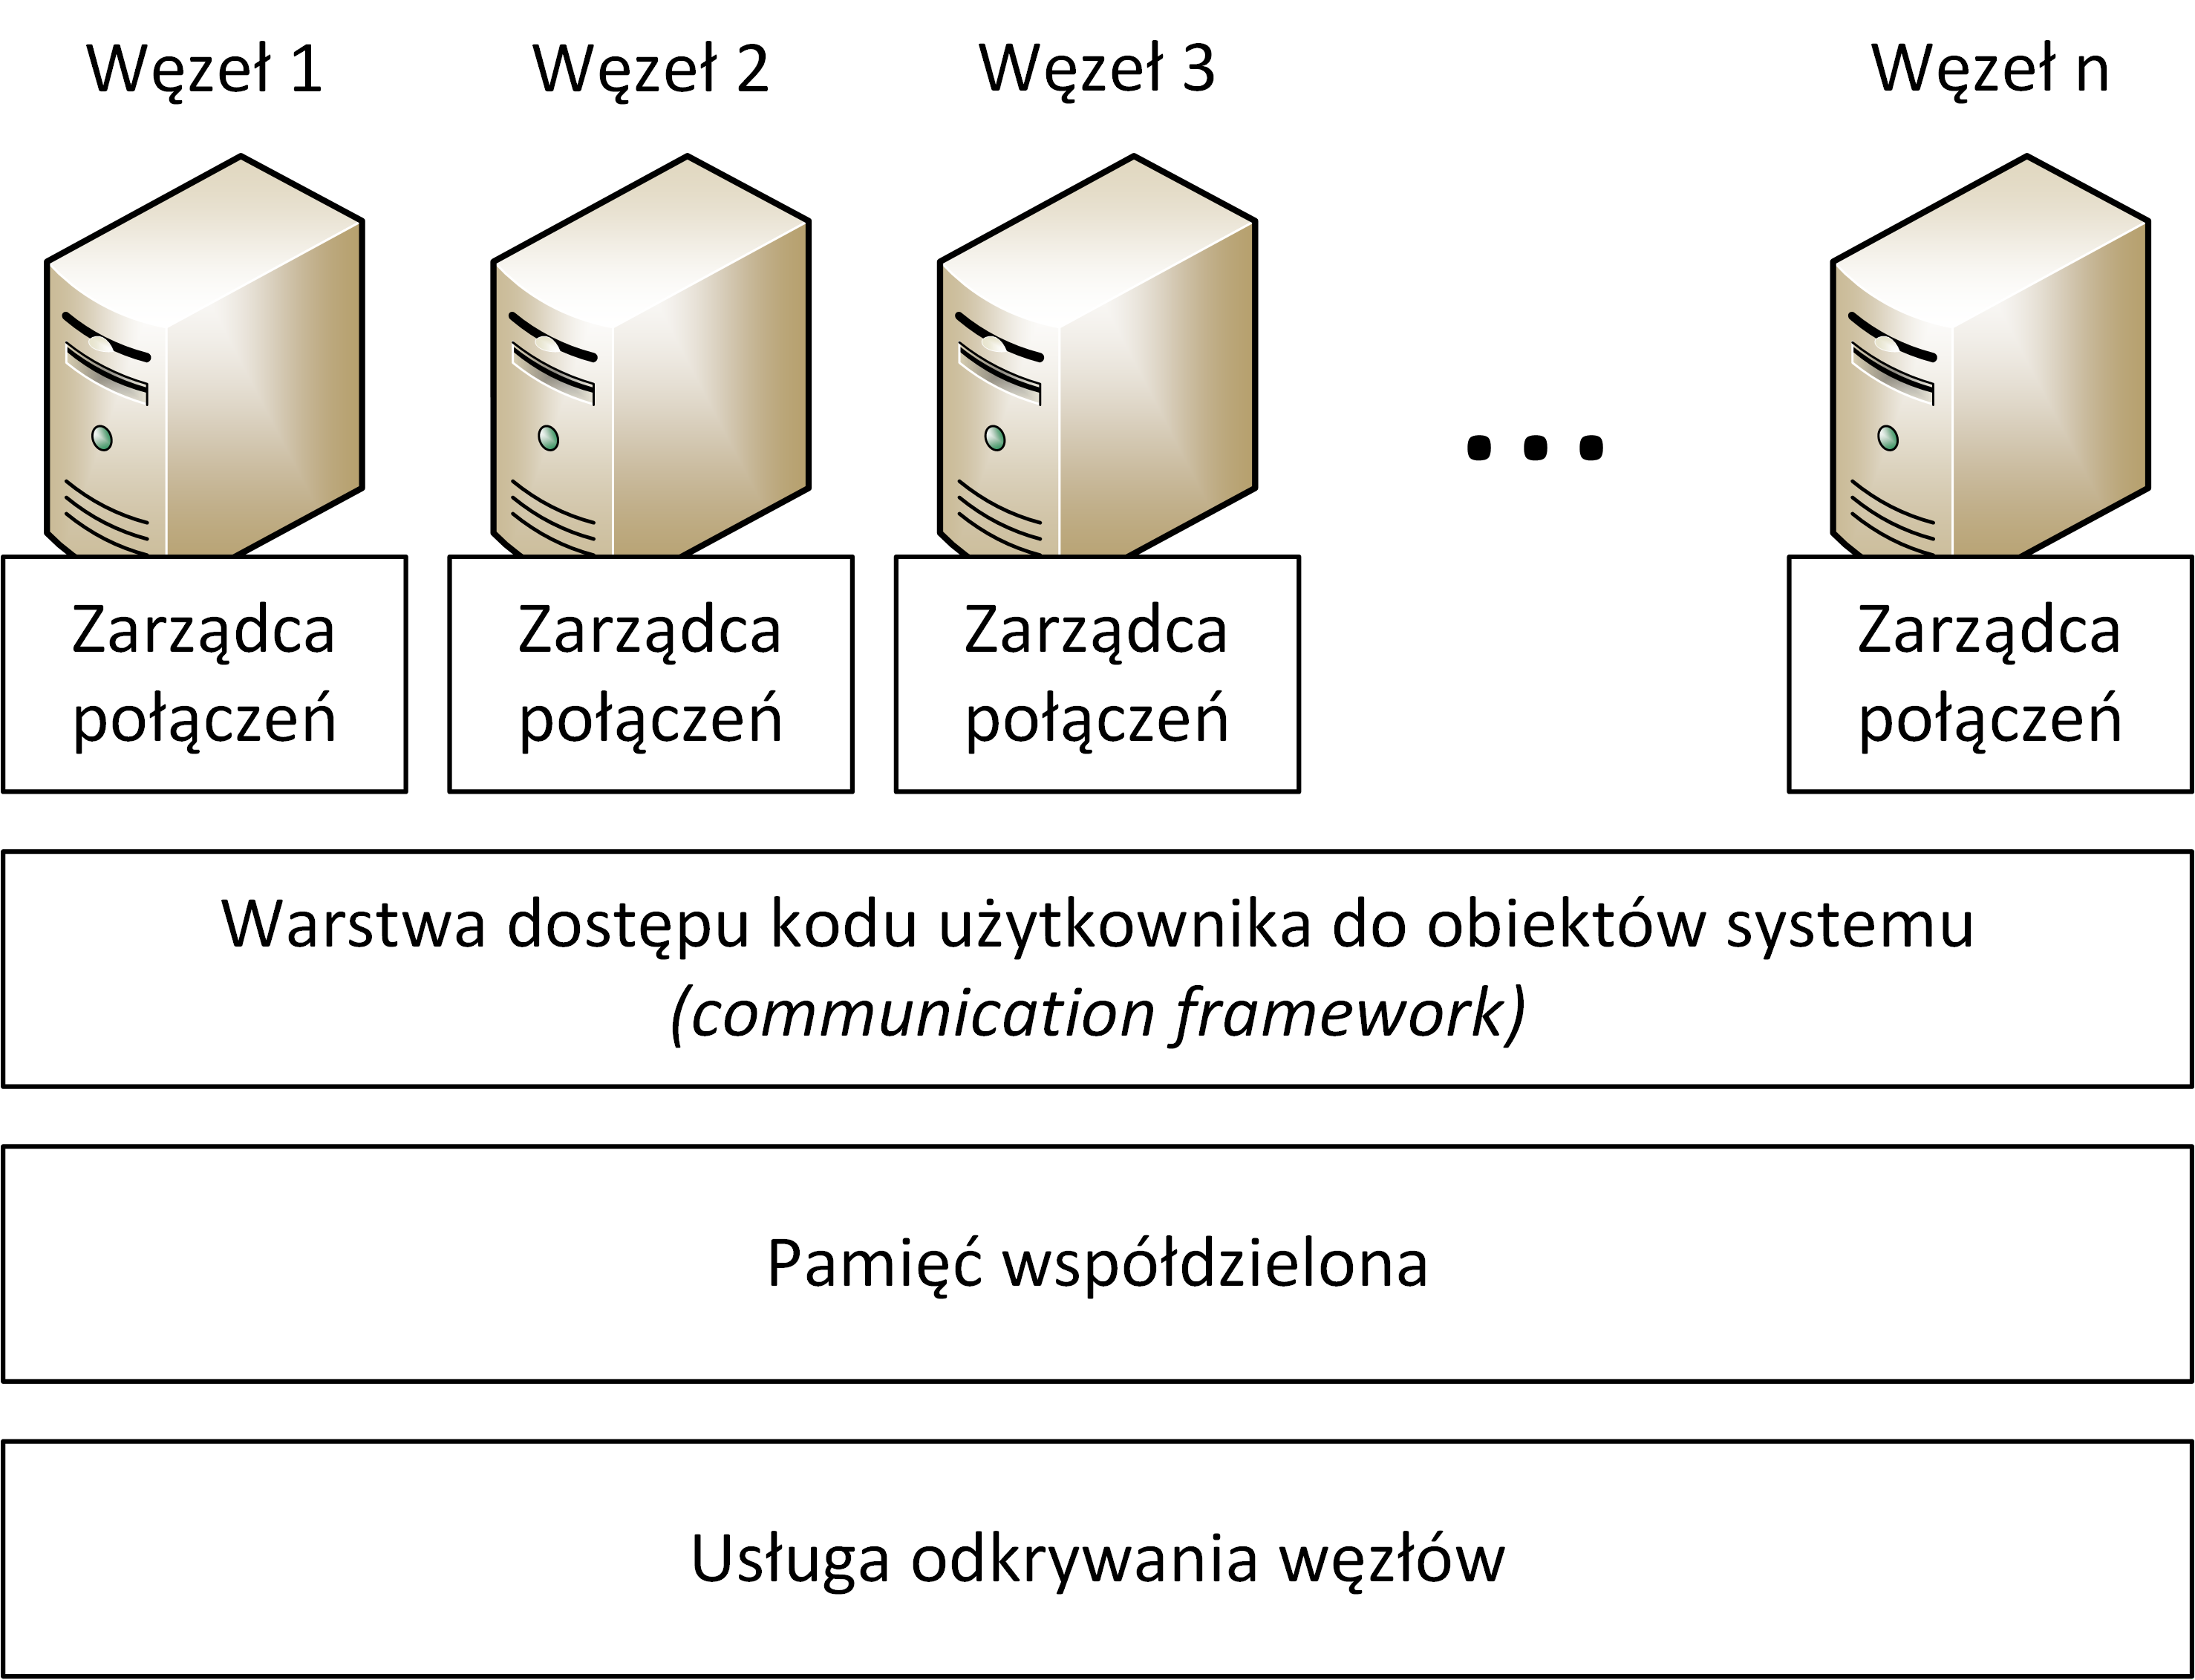
\includegraphics[scale=0.85]{images/schemat-systemu}\protect\caption{\label{fig:background-schemat-systemu}Schemat architektury systemu}
\end{figure}



\section{Usługa odnajdywania węzłów}

Jednym z podstawowych założeń jest posiadanie przez wszystkie węzły
w systemie lokalnej wiedzy o wszystkich innych węzłach obecnych w
klastrze. Informacje dotyczące stanu poszczególnych węzłów są dostarczane
przez \dcsname{usługę odnajdywania węzłów}. Usługa ta powinna
obsługiwać sytuację rejestracji oraz wyrejestrowania się węzłów. System
z założenia abstrahuje od sposobu realizacji tej usługi (czy będzie
to system scentralizowany, czy rozproszony np. oparty na algorytmie
plotkującym). W związku z pełnioną rolą, \dcsname{usługa odnajdywania węzłów}
jest kluczowym elementem przy implementacji wykrywania awarii węzłów
w klastrze. Nowe węzły muszą zarejstrować się w usłudze. Po rejestracji
są one monitorowane dopóki nie opuszczą klastra i wyrejestrują się
lub ulegną awarii. Niedostępne węzły -- tzn. takie, które nie odpowiedziały
na zapytanie w określonym czasie -- są usuwane z klastra.
\begin{defn}
~

\noindent \label{def:background-Usluga-odnajdywania-wezlow}\dcsstrong{Usługa odnajdywania węzłów}
to system umożliwiający węzłom odnajdywanie się wzajemnie w sieci
i łączenie w klaster obliczeniowy.
\end{defn}

\subsection{Zarządca połączeń}

Każdy węzeł powinien przechowywać lokalnie obraz klastra, aby w momencie,
kiedy zajdzie potrzeba zlecenia zadania jednemu ze \dcsname{zdalnych wykonawców}
nie musiał odpytywać \dcsname{usługi odnajdywania węzłów}. Tym
zadaniem zajmuje się \dcsname{zarządca połączeń}. Przechowuje
on też dodatkowe informacje, które mogą zostać wykorzystane przez
\dcsname{planistę}, takie jak statystyki obciążenia węzłów.
\begin{defn}
~

\noindent \dcsstrong{Zarządca połączeń} to klient usługi odnajdywania
węzłów, który odpowiada za rejestrowanie, wyrejestrowywanie i przechowywanie
lokalnego obrazu stanu klastra na każdym z węzłów.
\end{defn}

\section{Wątek rozproszony}

Specyfika systemu Bluepath wymaga rozróżnienia wątku systemu operacyjnego
oraz \dcsname{wątku rozproszonego} rozumianego jako jednostki przetwarzania
w systemie. \dcsname{Wątek rozproszony} jest tworzony na podstawie
statycznej metody, która przyjmuje dowolną, liczbę parametrów i zwraca
wartość. Wynik przechwytywany jest przez środowisko i udostępniany
do odczytu na węźle, który zlecił wykonanie wątku. Rozproszony wątek
może zostać wykonany na dowolnym węźle obliczeniowym oraz uruchamiać
kolejne rozproszone wątki. Decyzja o wyborze miejsca wykonania wątku
podejmowana jest z wykorzystaniem lokalnej wiedzy o stanie klastra
przez \dcsname{planistę}. Wątek rozproszony musi wykonać się w całości
na jednym z węzłów -- nie ma możliwości wstrzymania przetwarzania,
przeniesienia wątku razem z aktualnym stanem i~wznowienia obliczeń
na innym węźle.
\begin{defn}
~

\noindent \label{def:background-Rozproszony-watek}\dcsstrong{Wątek rozproszony}
reprezentuje jednostkę przetwarzania w systemie. Opakowuje fragment
kodu, który może być wykonany na dowolnym węźle obliczeniowym.
\end{defn}

\subsection{Problem detekcji zakończenia}

W punkcie \ref{sub:background-Problem-detekcji-zakonczenia} zasygnalizowano
konieczność zaproponowania rozwiąznia problemu detekcji zakończenia.
\dcsname{Wątki rozproszone} tworzą drzewiastą strukturę przetwarzania
-- można ją określić mianem modelu dyfuzyjnego. Wyróżniamy tutaj inicjatora
przetwarzania w korzeniu logicznego drzewa oraz jego następniki --
procesy potomne, które ponadto mogą inicjować kolejne procesy. Użytkownik
musi zapewnić, że proces-rodzic nie zakończy się, dopóki nie zakończą
się jego procesy-dzieci korzystając z przeznaczonej do tego metody.


\section{Wykonawca}

W celu ograniczenia liczby zadań pełnionych przez \dcsname{wątek rozproszony}
zdefiniowano \dcsname{wykonawcę} -- element odpowiedzialny za wykonywanie
wątków. Zastosowanie takiej abstrakcji pozwala potraktować przetwarzanie
lokalne oraz zdalne w podobny sposób. Specjalizacje -- \dcsname{lokalny wykonawca}
i \dcsname{zdalny wykonawca} -- wynikają z potrzeby realizacji innej
logiki w przypadku wykonania kodu na lokalnej i zdalnej maszynie. 


\subsection{Lokalny wykonawca}

Wszystkie wątki wykonywane lokalnie (zarówno te które pochodzą z lokalnego
węzła jak i te zlecone przez inny węzeł) są zarządzane przez \dcsname{lokalnych wykonawców}.
Do zadań \dcsname{lokalnego wykonawcy} należą:
\begin{itemize}
\item rozpoczęcie przetwarzania, 
\item przekierowanie parametrów, 
\item przechwycenie wyjątków,
\item udostępnienie wyników wyższym warstwom po zakończeniu przetwarzania.\end{itemize}
\begin{defn}
~

\noindent \dcsstrong{Lokalny wykonawca} to obiekt, który odpowiada
za faktyczne wykonanie otrzymanego zadania.
\end{defn}

\subsection{Zdalny wykonawca}

Reprezentacją zdalnego uruchomienia \dcsname{wątku rozproszonego}
jest obiekt \dcsname{zdalnego wykonawcy}. Zleca on wykonanie zadania
węzłowi wybranemu przez \dcsname{planistę} oraz monitoruje stan
wykonania zadania (zakończenie, wystąpienie błędów). Jest on również
odpowiedzialny za odebranie wyniku przetwarzania i udostępnienie go
do odczytu na węźle zlecającym zadanie.
\begin{defn}
~

\noindent \dcsstrong{Zdalny wykonawca} to obiekt, który odpowiada
za zlecenie wykonania zadania na zdalnej maszynie.
\end{defn}

\section{Planista}

Elementem systemu decydującym o wyborze miejsca wykonywania \dcsname{wątku rozproszonego}
jest \dcsname{planista}. Każda jego realizacja musi być oparta na
zdefiniowanym interfejsie. Dzięki temu użytkownik może przygotować
własną implementację \dcsname{planisty} dostosowaną do prowadzonego
przetwarzania lub wybrać jedną z dostarczonych razem z biblioteką.
\begin{defn}
~

\noindent \dcsstrong{Planista} odpowiada za wybór węzła, do którego
wysłane zostanie zlecenie wykonania zadania. Realizuje zdefiniowaną
strategię szeregowania zadań w klastrze.
\end{defn}

\section{Pamięć rozproszona}

\label{sec:concept-Rozproszona-pami=000119=000107-wsp=0000F3=000142dzielona}Często
w ramach przetwarzania rozproszonego zachodzi potrzeba przesyłania
danych między węzłami. W celu jej zrealizowania, jako część biblioteki
\dcsname{Bluepath}, dostarczana jest abstrakcja \dcsname{pamięci rozproszonej}.
Umożliwia ona synchronizację i wymianę danych między działającymi
wątkami. Zaleca się jednak myślenie i korzystanie z~niej jako pamięci
masowej, ponieważ koszt dostępu do niej może być znacznie wyższy niż
do pamięci operacyjnej. W szczególności nie należy jej mylić z DSM
opisaną w~punkcie \ref{sub:background-DSM}.
\begin{defn}
~

\noindent \label{def:concept-Pamiec-rozproszona}\dcsstrong{Pamięć rozproszona}
to pamięć dostępna dla wszystkich węzłów, przez którą mogą wymieniać
się danymi.
\end{defn}
Implementacja pamięci rozproszonej nie była przedmiotem niniejszej
pracy. Zdecydowano się zastosować jedno z istniejących rozwiązań spełniających
następujące założenia:
\begin{itemize}
\item silna spójność danych -- wszystkie węzły odczytują zawsze tę samą,
najbardziej aktualną wartość,
\item dostępność mechanizmów umożliwiających realizację operacji o semantyce
atomowego porównania i zapisu (ang.~\dcsemph{test and set}) lub
atomowego odczytu i zapisu.
\end{itemize}
Warto zauważyć, że zgodnie z definicją \ref{def:concept-Pamiec-rozproszona}
pod pojęciem \dcsname{pamięci rozproszonej} będziemy rozumieć pamięć,
która jest udostępniana przez co najmniej jeden węzeł i~umożliwia
współdzielenie danych między wszystkimi węzłami obliczeniowymi w~klastrze.

W \dcsname{pamięci rozproszonej} zastosowano klucze -- unikalne
ciągi znaków -- jednoznacznie identyfikujące dane. W trakcie projektowania
\dcsname{pamięci rozproszonej} nie przewidziano zapewnienia hierarchii
kluczy. Tego typu mechanizm, choć przydatny w~pewnych przypadkach,
może zostać dostarczony przez nadbudowane nad \dcsname{pamięcią rozproszoną}
przez użytkownika abstrakcje. Aby zapewnić wysoką użyteczność oraz
możliwość rozbudowy \dcsname{pamięci rozproszonej}, w podstawowym
interfejsie przewidziane zostały następujące operacje:
\begin{itemize}
\item zapis (ang.~\dcsemph{store}) -- operacja zapisująca dane; w przypadku
gdy podany klucz już istnieje operacja nie powiedzie się,
\item zapis lub aktualizacja (ang.~\dcsemph{store or update}) -- operacja
zapisująca dane; w~przypadku gdy podany klucz istnieje, wartość zostanie
nadpisana,
\item aktualizacja (ang.~\dcsemph{update}) -- operacja aktualizująca dane
-- powiedzie się tylko wtedy, gdy podany klucz został wcześniej utworzony
w \dcsname{pamięci rozproszonej},
\item pobranie (ang.~\dcsemph{retrieve}) -- operacja pobierająca dane
-- powiedzie się tylko wtedy gdy podany klucz został wcześniej utworzony,
\item usunięcie (ang.~\dcsemph{remove}) -- operacja usuwająca dane --
powiedzie się tylko wtedy gdy podany klucz został wcześniej utworzony
w \dcsname{pamięci rozproszonej}.
\end{itemize}
Operacje te, choć wystarczające w większości zastosowań, zostały rozwinięte
o odpowiedniki operujące jednocześnie na grupach kluczy -- zostały
one opisane w \ref{sub:Koncepcja-Operacje-zbiorcze}.

Dzięki tak zdefiniowanej semantyce operacji, na podstawie \dcsname{pamięci rozproszonej}
można również zbudować bardziej złożone mechanizmy, takie jak \dcsname{zamki rozproszone}.
Zamki są wbudowanym mechanizmem w proponowanej bibliotece i są dostępne
poprzez interfejs \dcsname{rozszerzonej pamięci rozproszonej}, który
został opisany w punkcie \ref{sub:Koncepcja-Zamki-rozproszone}.
\begin{defn}
~

\noindent \dcsstrong{Rozszerzona pamięć rozproszona }to pamięć
rozproszona (def. \ref{def:concept-Pamiec-rozproszona}), która dodatkowo
udostępnia abstrakcję zamków.
\end{defn}

\subsection{Rozproszone struktury danych i obiekty}

\label{sub:----Koncepcja-wspoldzielone-struktury-danych}\dcsname{Pamięć rozproszona}
-- pomimo tego, że zapewnia operacje niezbędne do komunikacji w trakcie
przetwarzania -- może okazać się mechanizmem o zbyt niskim poziomie
abstrakcji. W związku z tym biblioteka dostarcza struktury danych
i obiekty oparte na \dcsname{pamięci rozproszonej}: listę, słownik
oraz licznik.


\subsubsection*{Lista}

Głównym zadaniem \dcsname{listy rozproszonej} jest przechowywanie
i udostępnianie listy obiektów dostępnej w każdym \dcsname{wątku rozproszonym},
który zna jej identyfikator. Lista ta zachowuje zgodność na poziomie
interfejsu z listą dostarczaną przez środowisko .NET Framework. Podstawowe
scenariusze wykorzystania \dcsname{listy rozproszonej} nie powinny
wymagać stosowania dodatkowych mechanizmów synchronizacji.


\subsubsection*{Słownik}

Oprócz listy, często wykorzystywaną strukturą danych jest słownik.
\dcsname{Słownik rozproszony} pozwala użytkownikowi na współdzielenie
między wątkami kolekcji typu klucz-wartość. Jednocześnie zapewnia
poprawność wykonania współbieżnych operacji, np. atomowego dodania
nowego klucza oraz zarejestrowania go w wewnętrznym indeksie kluczy.
Podobnie jak lista rozproszona słownik identyfikowany jest przez ciąg
znaków, który musi być znany wszystkim wątkom chcącym uzyskać do niego
dostęp.


\subsubsection*{Licznik}

\label{par:koncepcja-distributed-counter}Jedną z podstawowych struktur
rozproszonych jest \dcsname{licznik rozproszony}. Oprócz standardowych
operacji odczytu i ustawienia wartości, umożliwia on także atomowe
pobranie i zwiększenie wartości. 

Obiekt ten może być wykorzystany jako generator unikalnych kluczy
lub do dynamicznego podziału kolekcji na fragmenty -- każdy \dcsname{wątek rozproszony}
może pobierać wartość licznika i jednocześnie zwiększać jego wartość
o $n$. W ten sposób rezerwuje sobie $n$ obiektów począwszy od odczytanej
wartości identyfikatora i każdy z wątków może operować na rozłącznym
zbiorze obiektów.


\subsection{Operacje zbiorcze\label{sub:Koncepcja-Operacje-zbiorcze}}

Głównym kosztem przetwarzania rozproszonego są narzuty komunikacyjne.
Wykonywanie $n$ żądań w celu pobrania $n$ elementów z \dcsname{pamięci rozproszonej}
jest wysoce nieefektywne. W celu zminimalizowania kosztu komunikacji,
dla każdej operacji na \dcsname{pamięci rozproszonej} zdefiniowano
jej odpowiednik przyjmujący jako parametr zbiór kluczy. Dodanie tego
typu operacji pozwoli użytkownikowi w znaczący sposób zwiększyć efektywność
swojego przetwarzania (np. poprzez jednorazowe pobranie do pamięci
lokalnej przetwarzanych danych).
\begin{defn}
~\label{def:concept-Operacje-zbiorcze-def}

\noindent \dcsstrong{Operacje zbiorcze} (ang.~\dcsemph{bulk operations})
to operacje wykonywane jednocześnie na grupie obiektów o podobnych
właściwościach znajdujących się w pamięci rozproszonej.
\end{defn}

\subsection{Zamki rozproszone\label{sub:Koncepcja-Zamki-rozproszone}}

Przetwarzanie rozproszone oparte na \dcsname{wątkach rozproszonych},
podobnie jak przetwarzanie równoległe, może wymagać zastosowania sekcji
krytycznych. Operacje na \dcsname{pamięci rozproszonej} zostały
zdefiniowane w taki sposób, aby możliwe było stworzenie \dcsname{zamków rozproszonych}
-- współdzielonych przez wszystkie węzły w klastrze (w~odróżnieniu
od zamków istniejących jedynie w obrębie jednego procesu bądź jednego
komputera) -- opartych o ten mechanizm. W związku z tym tworzenie
i zarządzanie \dcsname{zamkami rozproszonymi} jest częścią obowiązków
\dcsname{rozszerzonej pamięci rozproszonej}. 

Ponieważ reszta biblioteki nie polega na sposobie implementacji zamków,
a jedynie na gwarancjach jakie oferują, mogą one zostać zaimplementowane
przez użytkownika w oparciu o mechanizmy niezwiązane z \dcsname{pamięcią rozproszoną}.

\noindent %
\begin{minipage}[t]{1\textwidth}%
\begin{defn}
~

\dcsstrong{Zamek rozproszony} to zamek, który jest współdzielony
przez wszystkie węzły w~klastrze.\end{defn}
%
\end{minipage}


\section{Logowanie zdarzeń}

W celu umożliwienia przeglądu przebiegu przetwarzania system udostępnia
mechanizmy do zapisu historii zdarzeń -- zarówno tych wewnętrznych
jak i zachodzących w kodzie użytkownika. Opcjonalnie, korzystając
z abstrakcji \dcsname{listy rozproszonej}, log jest zbierany w \dcsname{pamięci rozproszonej}.
Dzięki temu użytkownik nie musi samodzielnie zbierać logów z wszystkich
węzłów w klastrze -- wystarczy, że na jednym z nich zmaterializuje
zawartość \dcsname{listy rozproszonej} do pliku w celu dalszego przetwarzania
i~wizualizacji np. w narzędziach służących do eksploracji procesów.


\section{Obsługa awarii}

\label{sec:concept-Obsluga-awarii}W obecnej wersji systemu nie przewiduje
się mechanizmów odtwarzania i kontynuowania przetwarzania w przypadku
awarii jednego lub większej liczby węzłów. Temat ten może być przedmiotem
dalszych prac (por. punkt \ref{sub:conclusions-Obsluga-awarii}).


\chapter{Implementacja}

\label{chap:implementation}Projekt systemu zakładał napisanie go
w języku C\# w środowisku .NET Framework 4.5~\cite{Microsoft.NET}
i umożliwienie wykonywania kodu użytkownika z bibliotek skompilowanych
do kodu zarządzalnego dla .NET Framework w wersji nie nowszej niż
4.5. Testy wykonania kodu użytkownika zostały przeprowadzone z użyciem
aplikacji napisanych w językach C\# oraz F\#. 

System Bluepath działa na klastrze węzłów obliczeniowych. Na każdym
węźle musi zostać uruchomiona binarnie zgodna wersja aplikacji (w
stopniu umożliwiającym wykonanie dowolnej metody z dowolnej klasy
będącej częścią procesu za pomocą zserializowanego uchwytu otrzymanego
w ramach zlecenia pod pewnymi warunkami opisanymi w punkcie \ref{sec:implementation-Rozproszony-watek}).
W ramach jednego z wątków uruchamiana jest usługa nasłuchująca wywołań
-- zleceń, zapytań przychodzących od pozostałych węzłów.


\section{Komunikacja}

W sieci komunikacyjnej w warstwie transportowej działa protokół TCP
\cite{rfc675,rfc793,rfc1122}, który realizuje gwarancje niezawodnego
dostarczenia wiadomości z użyciem mechanizmu potwierdzeń i retransmisji
zgodnie z założeniem przyjętym w punkcie \ref{sub:concept-Komunikacja}
ppkt. 1. Komunikacja między węzłami została zrealizowana w modelu
RPC (pkt. \ref{def:background-RPC}) za pomocą WCF (pkt. \ref{def:background-WCF}).
Połączenia realizowane są za pomocą protokołu HTTP \cite{rfc2616},
a wiadomości są przesyłane zgodnie z protokołem SOAP~\cite{W3C-SOAP11,W3C-SOAP12-part0,W3C-SOAP12-part1},
co spełnia wymagania postawione w punkcie \ref{sub:concept-Komunikacja}
ppkt. 2. Z~uwagi na losowy wybór numerów portów założono, że na maszynach
nie działa zapora ogniowa (pkt. \ref{def:background-Firewall}) blokująca
połączenia przychodzące na portach o wysokich numerach. W sieci nie
może także działać mechanizm NAT, co uniemożliwiłoby realizację bezpośredniej
komunikacji między węzłami. 

Wątek nasłuchujący jest reprezentowany przez obiekt klasy \dcscode{BluepathListener}.
Wewnętrznie tworzy on instancję klasy faktycznie nasłuchującej na
losowym porcie na wiadomości zgodne z interfejsem \dcscode{IRemoteExecutorService},
który został przedstawiony na listingu \ref{lis:implementation-Interfejs-IRemoteExecutorService},
a szczegółowy opis protokołu znajduje się w punkcie \ref{sec:implementation-Wykonawca}
poświęconym \dcsname{wykonawcom}. Dokonywana jest też rejestracja
w \dcsname{usłudze odnajdywania węzłów}. Jeżeli w ramach jednego
procesu zostanie utworzone kilka instancji klasy \dcscode{BluepathListener}
każda z nich będzie nasłuchiwała na innym porcie i posiadała własną
kolekcję \dcsname{lokalnych wykonawców}. Lista znanych \dcsname{zdalnych wykonawców}
jest współdzielona w ramach procesu przez wszystkie wątki nasłuchujące. 

W systemie każdy węzeł może komunikować się z dowolnym innym, o ile
zna jego adres IP i numer portu, pod którym działa usługa. Komunikaty,
zarówno wywołania (ang.~\dcsemph{request}) jak i wywołania zwrotne
(ang.~\dcsemph{callback}), mają charakter asynchroniczny. Istnieje
również możliwość wyłączenia wywołań zwrotnych i przełączenia systemu
w tryb pracy z odpytywaniem (ang.~\dcsemph{polling}). Wprowadza
on dodatkowe opóźnienia, co dyskwalifikuje go w przypadku prowadzenia
w klastrze faktycznych obliczeń, znajduje jednak zastosowanie w niektórych
scenariuszach realizowanych w~środowisku testowym.

\inputencoding{latin2}\begin{lstlisting}[caption={Interfejs IRemoteExecutorService},label={lis:implementation-Interfejs-IRemoteExecutorService},language={[Sharp]C},numbers=left]
[ServiceContract]
public interface IRemoteExecutorService
{
    [OperationContract]
    Guid Initialize(byte[] methodHandle);

    [OperationContract]
    void Execute(Guid eId, object[] parameters, ServiceUri callbackUri);

    [OperationContract]
    void ExecuteCallback(Guid eid, RemoteExecutorServiceResult executeResult);

    [OperationContract]
    RemoteExecutorServiceResult TryJoin(Guid eId);

    [OperationContract]
    PerformanceStatistics GetPerformanceStatistics();
}
\end{lstlisting}
\inputencoding{utf8}


\section{Usługa odnajdywania węzłów}

Obecna implementacja zawiera usługę odnajdywania węzłów zrealizowaną
w sposób scentralizowany, a każdy z węzłów podłączających się do klastra
musi znać adres IP i numer portu, pod którym działa \dcsname{usługa odnajdywania węzłów}.
Usługa udostępnia metody służące do zarejestrowania się węzła (\dcscode{Register}),
wyrejestrowania się węzła (\dcscode{Unregister}), pobrania listy
zarejestrowanych w klastrze węzłów (\dcscode{GetAvailableServices}),
oraz pobrania statystyk wydajności wszystkich węzłów w klastrze (\dcscode{GetPerformanceStatistics}).

\inputencoding{latin2}\begin{lstlisting}[caption={Interfejs ICentralizedDiscoveryService},language={[Sharp]C},numbers=left]
[ServiceContract]
public interface ICentralizedDiscoveryService
{
    [OperationContract]
    ServiceUri[] GetAvailableServices();

    [OperationContract]
    void Register(ServiceUri uri);

    [OperationContract]
    void Unregister(ServiceUri uri);

    [OperationContract]
    Task<Dictionary<ServiceUri, PerformanceStatistics>> GetPerformanceStatistics();
}
\end{lstlisting}
\inputencoding{utf8}


\section{Wątek rozproszony}

\label{sec:implementation-Rozproszony-watek}\dcscode{DistributedThread}
to klasa, której instancje reprezentują jednostkę przetwarzania w
systemie czyli \dcsname{wątek rozproszony} (patrz \ref{def:background-Rozproszony-watek}).
Wątek taki tworzony jest na podstawie delegatu \dcscode{Func} opakowującego
statyczną (nazwaną lub anonimową) metodę. Liczba parametrów wejściowych
takiej metody to maksymalnie 16 (jest to ograniczenie wprowadzone
przez deklaracje typu \dcscode{Func} dostępne w .NET Framework).
Wszystkie typy parametrów oraz typ zwracany muszą być oznaczone atrybutem
\dcscode{Serializable}. Przykład tworzenia i uruchamiania przez użytkownika
\dcsname{wątku rozproszonego} z użyciem domyślnego \dcsname{zarządcy połączeń}
i \dcsname{planisty} został przedstawiony na listingu \ref{lis:implementation-Tworzenie-i-uruchamianie-watku}.

Środowisko zakłada izolację pomiędzy wątkami: \dcsname{wątki rozproszone}
działające w~ramach jednego procesu-hosta nie mogą komunikować się
ze sobą poprzez pamięć operacyjną, a parametry, z którymi wywoływana
jest metoda są kopiowane do nowych instancji klas i struktur. Wyjątkiem
jest tutaj dostarczana przez środowisko \dcsname{pamięć rozproszona}.
W tym przypadku użytkownik powinien stosować dostarczone wraz z nią
mechanizmy synchronizacji. 

\begin{minipage}[t]{1\textwidth}%
\inputencoding{latin2}\begin{lstlisting}[caption={Tworzenie
i uruchamianie rozproszonego w±tku},label={lis:implementation-Tworzenie-i-uruchamianie-watku},language={[Sharp]C},numbers=left]
var thread = DistributedThread.Create(
    new Func<..., IBluepathCommunicationFramework, ...>((..., bluepath) => { 
        ...
        return ...; 
    }
)); 

thread.Start(...);
\end{lstlisting}
\inputencoding{utf8}%
\end{minipage}


\section{Wykonawca}

\label{sec:implementation-Wykonawca}Poniżej opisane zostały szczegóły
protokołu komunikacyjnego (rys. \ref{fig:implementation-Protokol-IRemoteExecutorService})
używanego przez węzły obliczeniowe oraz szczegóły implementacji \dcsname{wykonawców}.

\begin{figure}
\centering{}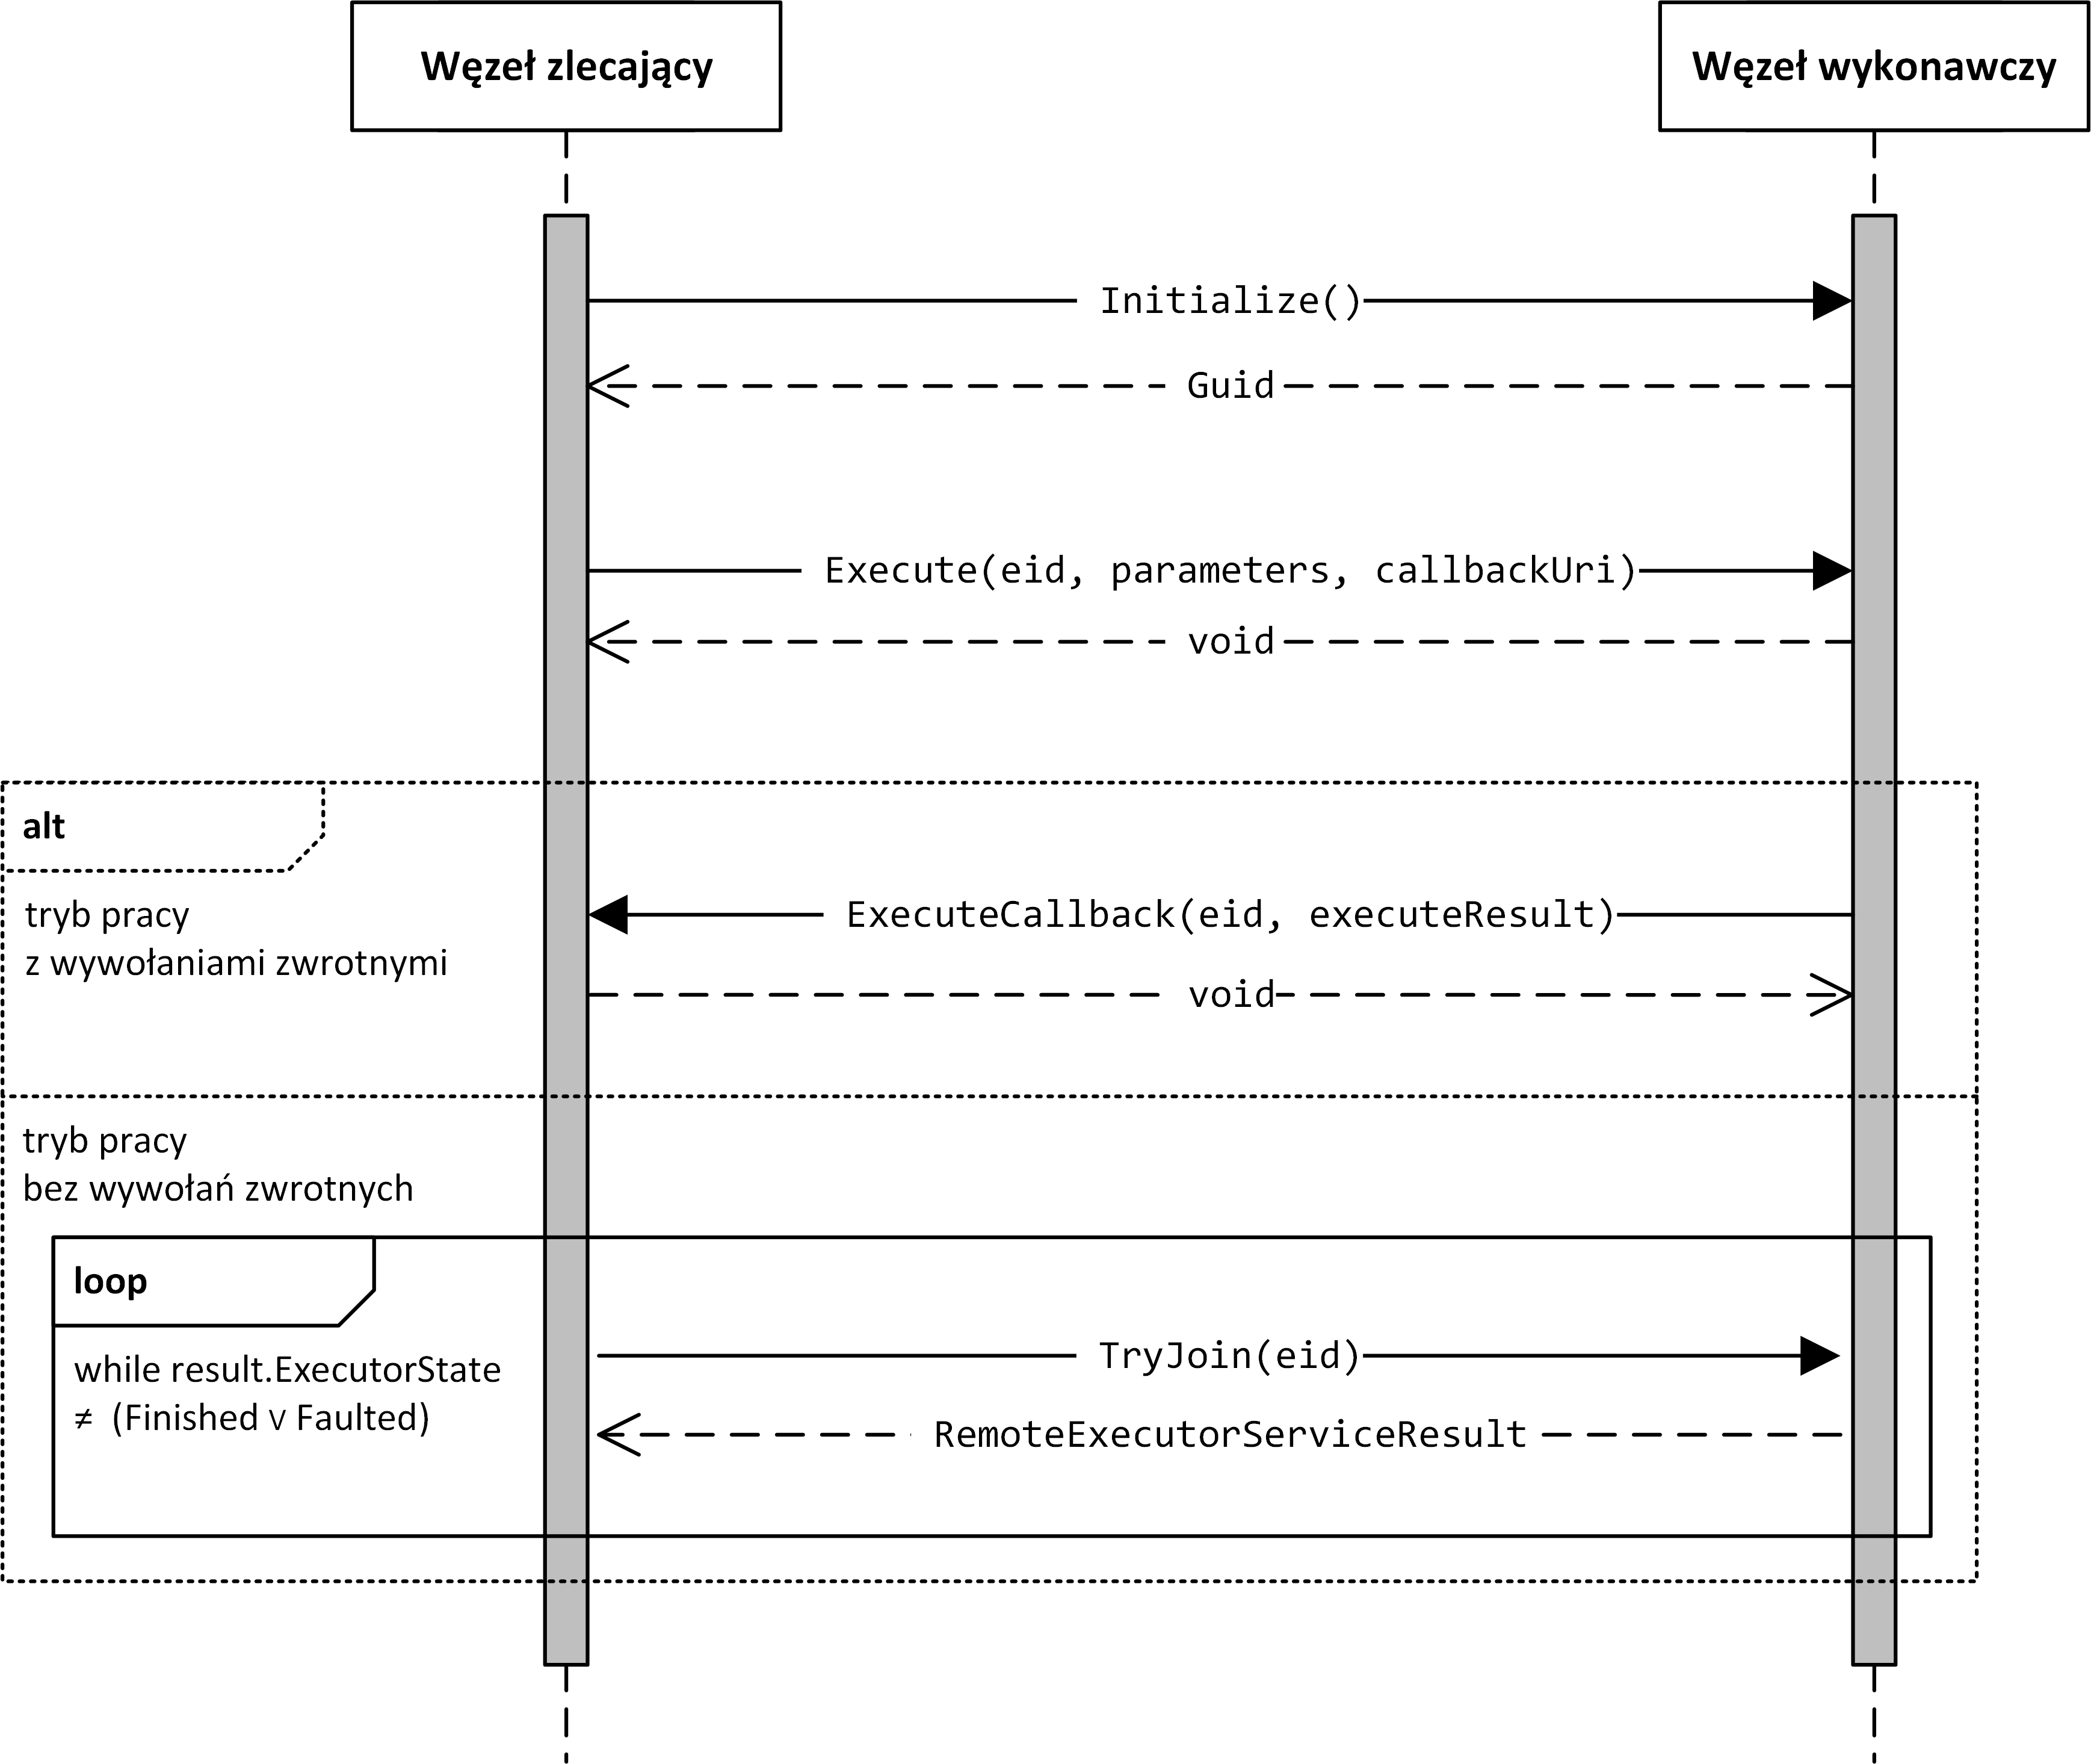
\includegraphics{images/diagram-protokolu}\protect\caption{\label{fig:implementation-Protokol-IRemoteExecutorService}Diagram
protokołu komunikacyjnego węzłów obliczeniowych}
\end{figure}



\subsection{Inicjalizacja}

Każdy wykonawca jest identyfikowany przez \dcscode{eid} (ang. \dcsemph{Executor ID})
-- unikalną 128-bitową liczbę (GUID, ang. \dcsemph{Globally Unique Identifier}),
przy czym instancja \dcsname{zdalnego wykonawcy} używa takiego samego
identyfikatora jak \dcsname{lokalny wykonawca}, który został zainicjowany
do wykonania kodu użytkownika. Wiadomość inicjująca wątek \dcscode{Initialize}
zawiera element \dcscode{methodHandle}, w którym przesyłany jest
zserializowany binarnie i zapisany w kodowaniu Base64 uchwyt do metody.
W odpowiedzi przesyłany jest identyfikator wykonawcy. Listing \ref{lis:implementation-SOAP-Initialize}
przedstawia w skróconej formie przykładową przechwyconą kopertę SOAP
z wiadomością \dcscode{Initialize}.

\inputencoding{latin2}\begin{lstlisting}[caption={Koperta SOAP -- inicjalizacja
zdalnego wykonawcy},label={lis:implementation-SOAP-Initialize},language=XML,numbers=left]
<s:Envelope xmlns:s="http://schemas.xmlsoap.org/soap/envelope/">
	<s:Body>
		<Initialize xmlns="http://tempuri.org/">
			<methodHandle>AAEAAAD/////AQAAAAAAAAAMAgAAAD9[...]==</methodHandle>
		</Initialize>
	</s:Body>
</s:Envelope>
\end{lstlisting}
\inputencoding{utf8}

Listing \ref{lis:implementation-SOAP-Initialize-decBase64} prezentuje
fragment uchwytu do metody po zdekodowaniu i usunięciu znaków spoza
drukowalnego zestawu symboli ASCII. DistributedPI to przykładowy program
opisany szerzej w punkcie \ref{sec:Przykladowe-zastosowania-liczba-pi}.
Uchwyt dotyczy metody anonimowej (stąd wygenerowana przez kompilator
nazwa \dcscode{b\_\_0}) zdefiniowanej w klasie \dcscode{Bluepath.DistributedPI.Program},
która jako parametr przyjmuje \dcscode{int} (\dcscode{System.Int32})
a typem zwracanym jest \dcscode{long} (\dcscode{System.Int64}). 

\inputencoding{latin2}\begin{lstlisting}[caption={Zdekodowany fragment
uchwytu do anonimowej metody},label={lis:implementation-SOAP-Initialize-decBase64},language=Assembler,numbers=left]
[...] System.Type[]
<RunTest>b__0 MBluepath.DistributedPI, Version=1.0.0.0, Culture=neutral, 
PublicKeyToken=null Bluepath.DistributedPI.Program
Int64 <RunTest>b__0(Int32) (System.Int64 <RunTest>b__0(System.Int32) 
System.UnitySerializationHolder Data	UnityType AssemblyName
\end{lstlisting}
\inputencoding{utf8}


\subsection{Przesłanie parametrów, wykonanie}

W kolejnej wiadomości, po inicjalizacji, węzeł zlecający przesyła
parametry wywołania metody. Przechwycona koperta z komunikatem \dcscode{Execute}
znajduje się na listingu \ref{lis:implementation-SOAP-Execute}. Warto
zauważyć, że ustawiona jest tutaj wartość pola \dcscode{callbackUri},
co~oznacza, że węzeł wywołujący otrzyma komunikat \dcscode{ExecuteCallback}
po zakończeniu przetwarzania po zdalnej stronie.

\inputencoding{latin2}\begin{lstlisting}[caption={Koperta SOAP -- przes³anie
paramterów},label={lis:implementation-SOAP-Execute},breaklines=true,language=XML,numbers=left]
<s:Envelope xmlns:s="http://schemas.xmlsoap.org/soap/envelope/">
	<s:Body>
		<Execute xmlns="http://tempuri.org/">
			<eId>6a3ff0e2-601b-4683-a163-7f6da037c762</eId>
			<parameters xmlns:a="http://schemas.microsoft.com/2003/10/Serialization/Arrays" xmlns:i="http://www.w3.org/2001/XMLSchema-instance">
				<a:anyType i:type="b:int" xmlns:b="http://www.w3.org/2001/XMLSchema">10000</a:anyType>
			</parameters>
			<callbackUri xmlns:a="http://schemas.datacontract.org/2004/07/Bluepath.Services" xmlns:i="http://www.w3.org/2001/XMLSchema-instance">
				<a:Address>http://192.168.0.7:51000/BluepathExecutorService.svc</a:Address>
				<a:BindingType>BasicHttpBinding</a:BindingType>
			</callbackUri>
		</Execute>
	</s:Body>
</s:Envelope>
\end{lstlisting}
\inputencoding{utf8}

Lokalny wykonawca szereguje wątki do wykonania używając dostarczonej
przez środowisko .NET Framework puli wątków (\dcscode{ThreadPool}).
Podejście to ma swoje wady -- tracona jest kontrola nad tak stworzonymi
wątkami, nie można ich przerwać lub sprawdzić ich stanu (uniemożliwia
to np. realizację detekcji zakleszczenia). Biblioteka Bluepath zapewnia,
że w przypadku, gdy w kodzie użytkownika wystąpi wyjątek, zostanie
on przechwycony, zserializowany i udostępniony wywołującemu wątkowi
do odczytu.


\subsection{Wywołanie zwrotne}

Po zakończeniu metody w trybie z wywołaniem zwrotnym, zdalna strona
przesyła wynik, ew. wyjątki oraz czas jaki zajęło przetwarzanie do
zlecającej maszyny. Przykładowy komunikat \dcscode{ExecuteCallback}
przedstawia listing \ref{lis:implementation-SOAP-ExecuteCallback}.

\noindent %
\begin{minipage}[t]{1\textwidth}%
\inputencoding{latin2}\begin{lstlisting}[caption={Koperta SOAP -- wywo³anie
zwrotne z wynikiem},label={lis:implementation-SOAP-ExecuteCallback},breaklines=true,language=XML,numbers=left]
<s:Envelope xmlns:s="http://schemas.xmlsoap.org/soap/envelope/">
	<s:Body>
		<ExecuteCallback xmlns="http://tempuri.org/">
			<eid>6a3ff0e2-601b-4683-a163-7f6da037c762</eid>
			<executeResult xmlns:a="http://schemas.datacontract.org/2004/07/Bluepath.Services" xmlns:i="http://www.w3.org/2001/XMLSchema-instance">
				<a:ElapsedTime>PT0.0125743S</a:ElapsedTime>
				<a:Error i:nil="true" xmlns:b="http://schemas.datacontract.org/2004/07/System"/>
				<a:ExecutorState>Finished</a:ExecutorState>
				<a:Result i:type="b:long" xmlns:b="http://www.w3.org/2001/XMLSchema">7857</a:Result>
			</executeResult>
		</ExecuteCallback>
	</s:Body>
</s:Envelope>
\end{lstlisting}
\inputencoding{utf8}%
\end{minipage}


\section{Planista}

Wraz z systemem dostarczone zostały następujące typy \dcsname{planistów}: 
\begin{itemize}
\item \dcscode{ThreadNumberScheduler} -- szereguje zadania na najmniej
obciążonym węźle pod względem liczby wykonywanych na nim wątków,
\item \dcscode{RoundRobinScheduler} -- szereguje zadania korzystając z
algorytmu cyklicznego (ang.~\dcsemph{round robin}) \cite{Tannenbaum-SOP}.
\end{itemize}
Wszystkie implementacje \dcsname{planisty} muszą implementować interfejs
\dcscode{IScheduler} dzięki czemu można zastosować implementację
\dcsname{planisty} dostosowaną do potrzeb przetwarzania i jest jednym
z elementów modułowości systemu. Poniżej zostały szczegółowo opisane
implementacje planistów dostarczonych z systemem. 


\subsection{Szeregowanie zadań w oparciu o obciążenie węzłów}

\label{sub:implementacja-szeregowanie-zadan-threadcount}Jednym z
podstawowych sposobów szeregowania zadań jest próba równomiernego
rozłożenia obciążenia węzłów. Zakładając, że wszystkie zadania mają
podobny rozmiar, jako miarę obciążenia konkretnego węzła można przyjąć
liczbę zadań, które są obecnie przetwarzane, lub oczekują na rozpoczęcie
przetwarzania.

W przykładowej implementacji dostarczanej wraz z biblioteką \dcsname{Bluepath}
informacje o obecnym obciążeniu węzłów są okresowo odświerzane prz
pomocy \dcsname{usługi odnajdywania węzłów}. W zależności od
szybkości tworzenia nowych \dcsname{wątków rozproszonych} oraz
częstotliwości odświerzania informacji o obciążeniu węzłów lokalne
dane mogą szybko stać się nieaktualne. Można ten efekt złagodzić poprzez
zwiększanie zapamiętanego obciążenia o wysłane na dany węzeł wątki.


\subsection{Szeregowanie zadań za pomocą algorytmu cyklicznego}

\label{sub:Implementacja-Szeregowanie-karuzelowy}W pewnych zastosowaniach
pewne zrównowarzenie obciążenia można osiągnąć poprzez zastosowanie
algorytmu cyklicznego. Algorytm ten nie wymaga pobierania informacji
o obciążeniu węzłów z \dcsname{usługi odnajdywania węzłów}, przez
co posiada mniejszy narzut komunikacyjny od algorytmów wymagających
tych informacji. 


\section{Pamięć rozproszona}

Ponieważ celem pracy nie było kompletne implementowanie pamięci rozproszonej,
skupiono się na wyborze istniejącego rozwiązania, które spełniałoby
wymagania zaprezentowane w punkcie \ref{sec:concept-Rozproszona-pami=000119=000107-wsp=0000F3=000142dzielona}.


\subsection{Rozważane rozwiązania }

\label{sub:implementation-Pamiec-rozproszona-rozwazane-rozwiazania}Początkowo
pod uwagę brane były następujące aplikacje:
\begin{itemize}
\item Memcached \cite{Memcached} -- system dostarczający rozproszoną pamięć
przechowującą dane w postaci par klucz-wartość. Nie znaleziono aktywnie
rozwijanego klienta dla platformy .NET,
\item Riak \cite{Riak} -- implementacja Amazon Dynamo \cite{Amazon-Dynamo},
odrzucony ze względu na brak API dla .NET Framework,
\item Polyphony \cite{Polyphony-blog-1,Polyphony-blog-2,Polyphony-blog-3,Polyphony-repo}
-- eksperymentalny projekt rozproszonej tablicy haszowej napisany
w języku F\#, nie wybrano ze względu na wczesnorozwojowy charakter
projektu,
\item Rhino DHT \cite{Rhino-DHT} -- implementacja rozproszonej tablicy
haszowej w języku C\#; posiada zależności od Rhino PHT (\dcsemph{persistent hash table})
\cite{Rhino-PHT} oraz Rhino Queues \cite{Rhino-Queues},
\end{itemize}
a w późniejszym okresie również:
\begin{itemize}
\item Redis \cite{Redis} -- system rozpowszechniany na licencji \dcsemph{open source}
przechowujący dane typu klucz-wartość.
\end{itemize}
Pierwszym wybranym rozwiązaniem było Rhino DHT, które było aktywnie
rozwijane przez rozpoznawalnego autora -- Ayende Rahiena. Niestety,
okazało się, że wersjonowanie danych nie zostało w pełni zaimplementowane
i nie było możliwe wykonanie atomowej operacji ,,odczytaj i zapisz'',
która była niezbędna do zrealizowania \dcsname{zamków rozproszonych}.
Szczegóły tego problemu zostały przedstawione w~punkcie \ref{par:problemy-rhino-dht}. 

Kolejnym rozwiązaniem wziętym pod uwagę był Redis -- system autorstwa
Salvatore Sanfilippo oraz Pietera Noordhuisa. Jest używany na co dzień
jako mechanizm pamięci podręcznej wielu serwisów internetowych (m.~in.
cała rodzina StackExchange) -- posiada przez to duże wsparcie i aktywnie
działającą społeczność. Redis potrafi działać zarówno jako pojedynczy
proces jak i w trybie master-slave, ponadto rozwijana jest wersja
rozproszona -- Redis Cluster. System ten posiada biblitekę dla .NET
Framework dostarczoną przez firmę StackExchange. Redis został napisany
dla rodziny systemów operacyjnych Linux, powstał jednak port tego
systemu do systemu operacyjnego Windows. Problemy, które napotkano
podczas uruchamiania usługi Redis (opisane w punkcie \ref{par:problemy-Windows-Redis})
udało się rozwiązać, przez co system ten został wykorzystany w ostatecznej
wersji pracy i w testach.


\subsection{Interfejsy pamięci rozproszonej}

Definicje \dcsname{pamięci rozproszonej} oraz \dcsname{rozszerzonej pamięci rozproszonej}
zostały sformalizowane w formie interfejsów odpowiednio \dcscode{IStorage}
oraz \dcscode{IExtendedStorage}. Interfejs \dcscode{IStorage} wymaga
implementacji metod do operacji na pojedynczych wartościach: \dcscode{Store},
\dcscode{StoreOrUpdate}, \dcscode{Update}, \dcscode{Retrieve} i
\dcscode{Remove} oraz operacji zbiorczych: \dcscode{BulkStore},
\dcscode{BulkStoreOrUpdate}, \dcscode{BulkUpdate}, \dcscode{BulkRetrieve}
i \dcscode{BulkRemove}. Semantyka tych operacji odpowiada operacjom
zdefiniowanym w punkcie \ref{sec:concept-Rozproszona-pami=000119=000107-wsp=0000F3=000142dzielona}.
Wszystkie operacje zdefiniowane w \dcsname{pamięci rozproszonej}
i \dcsname{rozszerzonej pamięci rozproszonej} pozwalają na bezpieczne
współbieżne wywołanie z wielu wątków (ang. \dcsemph{thread-safe}). 

Interfejs \dcscode{IExtendedStorage} rozszerza podstawowy interfejs
\dcscode{IStorage} o operacje pobrania i zwolnienia \dcsname{zamków rozproszonych}:
\dcscode{AcquireLock} (w wersji z limitem czasu oczekiwania na pobranie
zamka i bez) oraz \dcscode{ReleaseLock}. 


\subsection{Rozproszone struktury danych i obiekty}

Struktury danych i obiekty, które mogą być współdzielone między \dcsname{wątkami rozproszonymi}
zaimplementowane zostały w oparciu o \dcsname{pamięć rozproszoną},
zdefiniowaną za pomocą interfejsu \dcscode{IExtendedStorage} -- pozwoliło
to zastosować \dcsname{zamki rozproszone} w celu zapewnienia poprawności
przetwarzania -- współbieżny dostęp do rozproszonych struktur danych
i obiektów może być prowadzony zarówno z wątków jak i \dcsname{wątków rozproszonych}.
Każdy obiekt jest identyfikowany przez klucz będący łańcuchem znaków.
W przypadku listy czy słownika na podstawie klucza wywiedzione zostają
identyfikatory obiektów składających się na daną strukturę -- zamków,
metadanych i poszczególnych wartości. 


\subsubsection*{Lista}

Lista implementuje standardowy generyczny interfejs \dcscode{IList<T>}
z przestrzeni nazw \dcscode{System.Collections.Generic}. Próba pobrania
enumeratora zwraca obiekt klasy \dcscode{DistributedListEnumerator},
który umożliwia iterowanie po kolekcji. \dcsname{Lista rozproszona}
została rozszerzona o operację \dcscode{CopyPartTo} -- jest to odpowiednik
operacji \dcscode{CopyTo} (efektywnej operacji kopiowania całej zawartości
listy do wskazanej tablicy), który pozwala skopiować wybrany fragment
listy w sposób efektywny i atomowy. Operacja ta jest szczególnie przydatna
przy przetwarzaniu rozproszonym, gdzie dane znajdują się w wolnej
\dcsname{pamięci rozproszonej} (w stosunku do pamięci podręcznej),
a~każdy \dcsname{wątek rozproszony} przetwarza fragment danych.


\subsubsection*{Słownik}

Słownik implementuje standardowy generyczny interfejs \dcscode{IDictionary<TKey, TValue>}
z przestrzeni nazw \dcscode{System.Collections.Generic}. Próba pobrania
enumeratora zwraca obiekt klasy \dcscode{DistributedDictionaryEnumerator},
który umożliwia iterowanie po kolekcji. 


\subsubsection*{Licznik}

W wielu scenariuszach (przykładowy scenariusz opisany w \ref{par:koncepcja-distributed-counter})
przydatnym obiektem może być \dcsname{licznik rozproszony}. Zaimplementowana
klasa \dcscode{DistributedCounter} udostępnia następujące operacje: 
\begin{itemize}
\item \dcscode{GetValue} -- pobiera aktualną wartość licznika,
\item \dcscode{SetValue} -- ustawia podaną liczbę jako wartość licznika,
\item \dcscode{Increase} -- zwiększa wartość licznika o podaną wartość,
\item \dcscode{Decrease} -- zmniejsza wartość licznika o podaną wartość,
\item \dcscode{GetAndIncrease} -- atomowo pobiera aktualną wartość licznika
i zwiększa ją o~wskazaną liczbę, gdzie liczba o którą ma zostać zwiększony
licznik może być ujemna.
\end{itemize}

\subsection{Zamki rozproszone}

Odpowiednikiem definicji \dcsname{zamków rozproszonych} z punktu
\ref{sub:Koncepcja-Zamki-rozproszone} jest interfejs \dcscode{IStorageLock}.
Zdefiniowane w nim zostały następujące operacje:
\begin{itemize}
\item \dcscode{Acquire} -- operacja pobrania zamka. Posiada wariant, który
pozwala określić czas oczekiwania na pobranie zamka -- jeśli czas
ten zostanie przekroczony przed pobraniem zamka użytkownik dostanie
informację o niepowodzeniu i~będzie mógł kontynuować przetwarzanie.
Operacja pobrania zamka bez podania czasu oczekiwania jest blokująca
-- przetwarzanie będzie kontynuowane dopiero po pobraniu zamka,
\item \dcscode{Release} -- operacja zwolnienia zamka,
\item \dcscode{Wait} -- wykonanie tej operacji powoduje rozpoczęcie oczekiwania
na sygnał (ang.~\dcsemph{pulse}) od innego procesu. Wykonanie tej
operacji powoduje tymczasowe zwolnienie dostępu do zamka. Po otrzymaniu
sygnału proces próbuje ponownie pobrać zamek. Podobnie jak \dcscode{Acquire}
operacja ta posiada wariant, który pozwala określić czas oczekiwania
na sygnał,
\item \dcscode{Pulse} i \dcscode{PulseAll} -- wykonanie tych operacji
powoduje wysłanie sygnału do procesów oczekujących na operacji \dcscode{Wait}.
W pierwszym przypadku sygnał dotrze do conajmniej jednego oczekującego
procesu, a w drugim do wszystkich oczekujących procesów.
\end{itemize}
Interfejs \dcscode{IStorageLock} dziedziczy z interfejsu \dcscode{IDisposable}
-- sprawia to, że zamek można wykorzystać w podobny sposób jak słowo
kluczowe \dcscode{lock}, korzystając w tym celu z bloku \dcscode{using},
co przedstawiono na listingu \ref{lis:implementation-Realizacja-sekcji-krytycznej}.
Cechą bloku \dcscode{using} jest automatyczne wywołanie na jego końcu
operacji \dcscode{Dispose}, która w przypadku \dcsname{zamków rozproszonych}
powoduje zwolnienie zamka.

\noindent %
\begin{minipage}[t]{1\textwidth}%
\inputencoding{latin2}\begin{lstlisting}[caption={Realizacja
sekcji krytycznej z wykorzystaniem zamka rozproszonego},label={lis:implementation-Realizacja-sekcji-krytycznej},breaklines=true,language=bash,numbers=left]
using(var @lock = storage.AcquireLock("sampleLock"))
{
	// sekcja krytyczna
}
\end{lstlisting}
\inputencoding{utf8}%
\end{minipage}


\section{Logowanie zdarzeń}

\label{sec:implementation-Logowanie-zdarzen}Za zbieranie informacji
na temat zdarzeń zachodzących w systemie odpowiada klasa \dcscode{Log}
udostępniająca m. in. statyczne metody:
\begin{itemize}
\item \dcscode{ExceptionMessage} -- do logowania wyjątków,
\item \dcscode{TraceMessage} -- do logowania pozostałych zdarzeń.
\end{itemize}
Istnieje możliwość przekierowania wszystkich informacji do \dcsname{pamięci rozproszonej}.
W~tym celu należy ustawić flagę \dcscode{WriteToDistributedMemory}
oraz uzupełnić nazwę hosta \dcsname{pamięci rozproszonej} (\dcscode{DistributedMemoryHost}),
do którego ma odbywać się zapis. Warto zwrócić uwagę, że tryb pracy
ze zbieraniem historii zdarzeń w \dcsname{pamięci współdzielonej}
może istotnie ograniczać wydajność systemu. W celu zmaterializowania
zebranego logu udostępniona została metoda \dcscode{SaveXes}, która
zapisuje wszystkie zgromadzone w \dcsname{pamięci rozproszonej}
zdarzenia do pliku XML w formacie OpenXES. 

Implementacja zapisu zdarzeń do pliku XML została wykonana na podstawie
zmodyfikowanych plików XSD (pkt. \ref{def:background-XSD}) udostępnionych
wraz z biblioteką OpenXES \cite{OpenXES} w wersji 2.0 (przyczyny
i sposób modyfikacji został opisany w punkcie \ref{sub:problemy-Implementacja-standardu-OpenXES-z-XSD}).
Szkielet klas został wygenerowany przy użyciu narzędzia XML Schema
Definition Tool \cite{XML-Schema-Definition-Tool} (\dcscode{xsd.exe})
dostarczanego wraz ze środowiskiem programistycznym .NET Framework
4.5.1. Przykład użycia programu \dcscode{xsd.exe} został zaprezentowany
na listingu \ref{lis:implementation-Skrypt-generuj=000105cy-klasy-z-XSD}. 

\noindent %
\begin{minipage}[t]{1\textwidth}%
\inputencoding{latin2}\begin{lstlisting}[caption={Skrypt
generuj±cy klasy w jêzyku C\# na podstawie pliku XSD dla formatu OpenXES },label={lis:implementation-Skrypt-generuj=000105cy-klasy-z-XSD},breaklines=true,language=bash,numbers=left]
"c:\Program Files (x86)\Microsoft SDKs\Windows\v8.1A\bin\NETFX 4.5.1 Tools\xsd.exe" xes.xsd /classes /o:../Bluepath/Reporting/ 
"c:\Program Files (x86)\Microsoft SDKs\Windows\v8.1A\bin\NETFX 4.5.1 Tools\xsd.exe" xesext.xsd /classes /o:../Bluepath/Reporting/
\end{lstlisting}
\inputencoding{utf8}%
\end{minipage}

Wszystkie zdarzenia zachodzące w systemie zostały pogrupowane w tkw.
\dcsname{aktywności} (ang.~\dcsemph{activity}). Rodzaje aktywności
zachodzących w systemie zostały zdefiniowane w formie typu wyliczeniowego
\dcscode{Bluepath.Reporting.Log.Activity}, obejmuje on m. in.:
\begin{itemize}
\item \dcscode{Service\_is\_ready} -- zgłoszenie przez węzeł gotowości
do przyjęcia zleceń,
\item \dcscode{Local\_executor\_started\_running\_user\_code} -- rozpoczęcie
wykonywania kodu użytkownika w ramach rozproszonego wątku,
\item \dcscode{Local\_executor\_finished\_running\_user\_code} -- zakończenie
wykonywania kodu użytkownika na węźle,
\item \dcscode{Sending\_callback\_with\_result} -- wysłanie wywołania zwrotnego
z wynikiem działania wątku.
\end{itemize}
Wszystkie zdarzenia, które są mało istotne dla analizy procesu mogą
być grupowane w ramach aktywności \dcscode{Info} i powinny zostać
odfiltrowane w pierwszej fazie analizy. Jeżeli użytkownik chce użyć
własnej nazwy dla zdarzenia, może to zrobić korzystając z aktywności
\dcscode{Custom}, a właściwą nazwę przekazać jako parametr \dcscode{message}
do metody logowania zdarzeń. 

Format XES definiuje dla zdarzeń w logu \dcsname{zasób} (ang.~\dcsemph{resource})
-- w przypadku biblioteki \dcsname{Bluepath} wartością tego pola
jest zawsze wykonawca, który dokonał wpisu, korzystając z jego unikalnego
identyfikatora \dcscode{eid}. Implementacja zakłada możliwość skrócenia
zapisu do n ostatnich znaków składających się na identyfikator w celu
ułatwienia analizy przez człowieka. Może to potencjalnie wpłynąć na
fałszywe sklasyfikowanie różnych zasobów jako tego samego w wyniku
kolizji tak skonstruowanych identyfikatorów.

Zależności czasowe są istotną częścią analizy przebiegu procesu. Z
wykorzystaniem serwerów czasu implementujących protokół NTP (ang.
\dcsemph{network time protocol}) \cite{rfc5905} możliwe jest zsynchronizowanie
zegarów węzłów w klastrze z dokładnością do milisekund (przy dużych
odległościach od serwera czasu -- dziesiątek milisekund) \cite{Mills-NTP-IEEE-Trans}.
Może to być niewystarczające do jednoznacznego określenia porządku
zdarzeń. Klasa \dcscode{Log} zawiera flagę \dcscode{monotonicallyIncreasingLogTime},
której ustawienie uniemożliwia zapisanie dwóch zdarzeń z tym samym
znacznikiem czasowym poprzez realizowanie dodatkowych operacji podczas
zapisu do logu:
\begin{itemize}
\item pobranie \dcsname{zamka rozproszonego},
\item odczyt ostatnio zapisanej wartości znacznika czasowego z \dcsname{pamięci rozproszonej},
\item w przypadku gdy lokalna wartość znacznika jest mniejsza lub równa
odczytanemu, jest ona zamieniana na odczytaną wartość zwiększoną o
1 milisekundę,
\item zapis bieżącej wartości znacznika czasowego do \dcsname{pamięci rozproszonej},
\item zwolnienie \dcsname{zamka rozproszonego}.
\end{itemize}



\section{Interfejs do komunikacji z systemem}

Aby skorzystać z funkcji udostępnianych przez system (jak np. pobranie
identyfikatora \dcsname{wykonawcy} czy dostęp do \dcsname{pamięci rozproszonej})
wewnątrz \dcsname{wątku rozproszonego}, użytkownik musi uzyskać
przeznaczony do tego obiekt. System automatycznie wstrzykuje go do
metod jako jeden z parametrów -- wystarczy, by był on typu \dcscode{IBluepathCommunicationFramework}.
Użytkownika ma również możliwość zapisywania własnych zdarzeń zachodzących
w aplikacji do logu z użyciem opisanej w punkcie \ref{sec:implementation-Logowanie-zdarzen}
statycznej klasy \dcscode{Log}.


\section{Dystrybucja aplikacji w klastrze}

\label{sec:implementation-Skrypt-Send-Folder}PowerShell Remoting
\cite{PS-Remoting} to usługa umożliwiająca wykonanie na zdalnych
maszynach pojedynczych komend lub stworzenie pełnej zdalnej sesji
PowerShell. Automatyzacja procesu dystrybucji plików binarnych systemu
w klastrze została zrealizowana za pomocą zestawu skryptów: \dcspath{Send-Folder}
do przesyłania całych folderów i \dcspath{Send-File} do przesyłania
pojedynczych plików, z którego korzysta ten pierwszy. 

Skrypt do wysyłania pojedynczych plików został zaczerpnięty z książki
\cite{Windows-PowerShell-Cookbook}. Przyjmuje 3 parametry: ścieżkę
do pliku źródłowy znajdującego się na lokalnej maszynie, ścieżkę docelową
na zdalnej maszynie oraz referencję do obiektu zdalnej sesji. Plik
jest wczytywany do pamięci jako tablica bajtów, następnie jego transfer
odbywa się strumieniowo w blokach o rozmiarze 1 MB. Po zrekonstruowaniu
tablicy bajtów na zdalnej stronie jest ona zapisywana na dysk we wskazanej
lokalizacji.

Skrypt do wysyłania folderów przedstawiony na listingu \ref{lis:implementation-Send-Folder}
przyjmuje jako parametry: 
\begin{itemize}
\item adres zdalnego komputera (\dcscode{-server}), 
\item opcjonalnie port, na którym nasłuchuje usługa PowerShell Remoting
(\dcscode{-port}), 
\item nazwę użytkownika (\dcscode{-user}), 
\item hasło (\dcscode{-password}), 
\item ścieżkę do folderu źródłowego na lokalnej maszynie (\dcscode{-source}), 
\item oraz ścieżkę do folderu docelowego na zdalnej maszynie (\dcscode{-destination}). 
\end{itemize}
Skrypt tworzy obiekt zdalnej sesji uwierzytelniając się poprzez podaną
nazwę użytkownika i hasło. W celu uproszczenia etapu konfiguracji
środowiska, do wywołania metody \dcscode{New-PSSession} można dodać
przełącznik \dcscode{-SessionOption} z parametrem \dcscode{New-PSSessionOption -SkipCACheck}.
Opcja ta powoduje jednak obniżenie poziomu bezpieczeństwa poprzez
dopuszczenie niezaufanych certyfikatów maszyn. Następnie pobierana
jest lista plików we wskazanym lokalnym folderze i dla każdego z plików
wywoływany skrypt \dcspath{Send-File}. Pomijane przy tym są pliki
z symbolami (\dcspath{.pdb}), ponieważ ich rozmiar jest znaczący
w stosunku do rozmiaru plików samej aplikacji, a nie było konieczne
podłączanie \dcsemph{debuggera} do procesów pracujących na zdalnych
maszynach. Po zakończeniu przesyłania plików zdalna sesja jest zamykana.
Warto zauważyć, że skrypt \dcspath{Send-Folder} można wywołać wielokrotnie
przekazując w parametrze -server kolejne adresy maszyn, aby rozdystrybuować
pliki w całym klastrze.

\inputencoding{latin2}\begin{lstlisting}[caption={Skrypt przesy³aj±cy pliki ze
wskazanego folderu na zdaln± maszynê},label={lis:implementation-Send-Folder},language=bash,numbers=left]
param (
	[string]$server = $(throw "-server is required."),
	[int]$port = 5986,
	[string]$user = $(throw "-user is required."),
	[string]$password = $(throw "-password is required."),
	[string]$source = $(throw "-source is required."),
	[string]$destination = $(throw "-destination is required.")
)

$secPassword = ConvertTo-SecureString $password -AsPlainText -Force
$credential = New-Object System.Management.Automation.PSCredential($user, $secPassword)
$uri = New-Object System.Uri("https://" + $server + ":" + $port)

$session = New-PSSession -ConnectionUri $uri -Credential $credential

Get-ChildItem -Path $source -File | Foreach-Object {
	if ($_.Extension -ne ".pdb") {
		$target = $destination + $_.Name
		.\Send-File.ps1 $_.FullName $target $session
	}
}

Disconnect-PSSession $session
\end{lstlisting}
\inputencoding{utf8}


\chapter{Przykładowe zastosowania}

\label{chap:applications}W tym rozdziale przedstawione zostaną przykladowe
zastosowania systemu Bluepath. Na bazie \dcsname{wątków rozproszonych},
\dcsname{pamięci rozproszonej} i nadbudowanych nad nią abstrakcji
listy i słownika przygotowane zostały projekty:
\begin{itemize}
\item \dcsstrong{DLINQ} (ang.~\dcsemph{Distributed Language Integrated Query})
-- dostawca metod manipulacji kolekcji w sposób zgodny z obecnym już
w środowisku .NET dla standardowych, nierozproszonych kolekcji, 
\item \dcsstrong{MapReduce} -- abstrakcja specjalizowana do uruchamiania
zadań w modelu mapowania i redukcji z możliwością zlecania zadań bez
konieczności ponownej kompilacji systemu i dystrybuowania nowej wersji
plików wykonywalnych na węzły,
\item \dcsstrong{System uzupełniania wyrazów} -- system przygotowujący
na podstawie podanej kolekcji dokumentów bazę prefiksów, która jest
wykorzystywana do realizacji systemu podpowiedzi słów na podstawie
pierwszych liter wpisywanych przez użytkownika,
\item \dcsstrong{Obliczanie przybliżenia liczby $\pi$} -- algorytm obliczający
przybliżoną wartość liczby $\pi$, który umożliwił przeprowadzenie
testów porównawczych szybkości obliczeń w klastrze bez wykorzystania
\dcsname{pamięci rozproszonej} w stosunku do obliczeń prowadzonych
na pojedynczym węźle.
\end{itemize}

\section{DLINQ}

Jednym z przykładowych zastosowań biblioteki Bluepath jest Distributed
Language Integrated Query (DLINQ) -- zbiór metod roszerzających możliwości
operowania na kolekcjach bazowanych na \dcsname{pamięci rozproszonej}.
Obecna implementacja służy jako przykład (ang.~\dcsemph{proof of concept})
wykorzystania możliwości dostarczanych przez bibliotekę Bluepath i
dlatego dostarcza implementację podzbioru metod standardowego zestawu
LINQ:
\begin{itemize}
\item \dcscode{Select} -- operacja ta pozwala przetransformować obiekt,
np. wybierając jedynie podzbiór jego atrybutów, lub zmieniając typ
obiektu,
\item \dcscode{SelectMany} -- operacja podobna do \dcscode{Select} z tą
różnicą, że pojedynczy obiekt w wyniku transformacji zmieniany jest
w kolekcję obiektów, a powstałe w ten sposób kolekcje są łączone w
jedną,
\item \dcscode{Where} -- operacja ta pozwala wyfiltrować te obiekty, które
spełniają podany warunek,
\item \dcscode{GroupBy} -- operacja pozwalająca grupować obiekty według
zadanego klucza,
\item \dcscode{Count} -- operacja zliczające obiekty spełniające zadany
warunek. 
\end{itemize}
Operacje te mogą być wykonywane zarówno na dostarczonej z biblioteką
Bluepath liście rozproszonej (opisanej w \ref{sub:----Koncepcja-wspoldzielone-struktury-danych})
jak i na wszystkich obiektach implementujących interfejs \dcscode{IEnumerable}.
W drugim przypadku kolekcja źródłowa zostanie najpierw przetransformowana
do listy rozproszonej, a następnie poddana dalszemu przetwarzaniu.

Sposób wykorzystania rozszerzeń DLINQ jest wzorowany na Parallel Language
Integrated Query (PLINQ). Aby poddać kolekcję przetwarzaniu rozproszonemu
wykonujemy najpierw metodę rozszerzającą \dcscode{AsDistributed}.
Metoda ta posiada jeden obowiązkowy argument -- obiekt zapewniający
dostęp do \dcsname{pamięci rozproszonej}. Następnie na otrzymanym
z tej metody obiekcie można wykonywać operacje zdefiniowane w DLINQ.
Należy jednak mieć na uwadze, że operacje te podlegają założeniom
biblioteki Bluepath i funkcje podawane jako argumenty muszą być funkcjami
statycznymi. Na listingu \ref{lis:Transformacja-kolekcji-DLINQ} przedstawiono
przykładowy kod poddający kolekcję transformacji przy użyciu metody
\dcscode{Select}.

\inputencoding{latin2}\begin{lstlisting}[caption={Transformacja kolekcji przypomocy
metod dostarczonych w DLINQ},label={lis:Transformacja-kolekcji-DLINQ},breaklines=true,language={[Sharp]C},numbers=left]
var inputCollection = new List<double>(100);
...
var processedCollection = (from num in inputCollection.AsDistributed(storage) select Math.Sqrt(num)).ToList();
\end{lstlisting}
\inputencoding{utf8}

W implementacji DLINQ można wyróżnić 3 podstawowe klasy: \dcscode{DistributedQuery},
\dcscode{DistributedEnumerable} oraz \dcscode{UnaryQueryOperator}.
Zostały one dokładniej opisane w poniższych punktach.


\subsection{DistributedQuery}

W celu zapewnienia jednoznacznego rozróżnienia pomiędzy metodami LINQ,
oraz DLINQ wprowadzono klasę \dcscode{DistributedQuery}. Klasa ta
częściowo implementuje interfejs \dcscode{IEnumerable} zapewniając
powiązania pomiędzy metodami tego interfejsu. Stanowi ona bazę z której
wywodzą się wszystkie klasy realizujące poszczególne wywołania DLINQ
(np. \dcscode{Select}) co pozwala na wykonywanie tych samych metod
na instancjach różnych klas składowych DLINQ.


\subsection{DistributedEnumerable}

Statyczna klasa \dcscode{DistributedEnumerable} zawiera wszystkie
metody rozszerzające DLINQ. Każda z tych metod weryfikuje parametry
wejściowe w celu przekazania użytkownikowi zrozumiałych informacji
w przypadku podania błędnych parametrów. Następnie tworzona jest klasa
realizująca wywołanie DLINQ i zwracana użytkownikowi w celu dalszego
przetwarzania (samo wykonanie podobnie jak w LINQ następuje dopiero
wtedy gdy potrzebne są wyniki np. wywołanie metody \dcscode{ToList},
lub enumeracja).

Specjalną metodą rozszerzającą zaimplementowaną w klasie \dcscode{DistributedEnumerable}
jest metoda \dcscode{AsDistributed}. Służy ona przygotowaniu kolekcji
wejściowej do przetwarzania przez metody DLINQ. Jest to realizowane
poprzez opakowanie kolekcji wejściowej klasą \dcscode{DistributedEnumerableWrapper},
która przenosi zawartość kolekcji wejściowej do \dcsname{listy rozproszonej}
(wyjątkiem jest sytuacja, w której kolekcja wejściowa jest \dcsname{listą rozproszoną}).


\subsection{UnaryQueryOperator}

Klasą bazową dla klas implementujących metody DLINQ jest \dcscode{UnaryQueryOperator}.
Jest to klasa, która gromadzi wszystkie metody wspólne dla metod DLINQ
takich jak tworzenie \dcsname{wątków rozproszonych} z wykorzystaniem
ustawień przekazanych przez użytkownika w metodzie \dcscode{AsDistributed},
czy zebranie wyników przetwarzania z poszczególnych \dcsname{wątków rozproszonych}.
Nazwa \dcscode{UnaryQueryOperator} wynika z faktu, że wszystkie metody
DLINQ oparte na tej klasie operują na jednej kolekcji. W przypadku
implementacji metod takich jak \dcscode{Union} -- metoda odpowiadająca
za połączenie dwóch kolekcji -- należałoby stworzyć kolejne klasy,
np. \dcscode{BinaryQueryOperator}.


\section{MapReduce}

\label{sec:applications-MapReduce}W celu porównania pracochłonności
implementacji aplikacji z użyciem bibliteki Bluepath i bez niej przygotowane
zostały aplikacje do realizacji przetwarzania w modelu mapowania i
redukcji zarówno w środowisku Bluepath jak i bezpośrednio z~wykorzystaniem
platformy Windows Communication Foundation~\cite{MSDN:WhatIsWindowsCommunicationFoundation}.
Założeniem aplikacji było, by kod metod \dcscode{Map} i \dcscode{Reduce}
dostarczany był jako kod źródłowy w języku C\# w formie klasy implementującej
odpowiedni interfejs -- \dcscode{IMapProvider} lub \dcscode{IReduceProvider}
-- przedstawiony na listingu \ref{lis:applications-MapReduce-IMapProvider-IReduceProvider}
i składowany razem z danymi w~\dcsname{pamięci rozproszonej}. Kompilacja
kodu miała odbywać się na węzłach bezpośrednio przed wykonaniem metody,
do zrealizowania tego celu wybrana została biblioteka CS-Script~\cite{CS-Script}. 

\noindent %
\begin{minipage}[t]{1\textwidth}%
\inputencoding{latin2}\begin{lstlisting}[caption={Interfejsy
IMapProvider i IReduceProvider},label={lis:applications-MapReduce-IMapProvider-IReduceProvider},breaklines=true,language={[Sharp]C},numbers=left]
public interface IMapProvider 
{
   IEnumerable<KeyValuePair<string, string>> Map(string key, string value); 
}

public interface IReduceProvider 
{
   KeyValuePair<string, string> Reduce(string key, IEnumerable<string> values); 
}
\end{lstlisting}
\inputencoding{utf8}%
\end{minipage}


\subsection{Koordynator}

Główną klasą w aplikacji jest \dcsname{koordynator}, który pełni
rolę nadzorcy zadań (z tego powodu nazywany jest także \dcsemph{JobTrackerem}).
Jego zadaniem jest przydzielanie zdań mapowania i redukcji podległym
węzłom. Poniżej opisano jego implementacje z wykorzystaniem biblioteki
Bluepath jak i w oparciu bezpośrednio o technologię WCF.


\subsubsection*{Koordynator oparty o Bluepath}

W środowisku Bluepath jego zadanie sprowadzało się w pierwszej fazie
przetwarzania do uruchomienia \dcsname{wątków rozproszonych} w
liczbie odpowiadającej liczbe plików wejściowych, które były inicjowane
metodą, która:
\begin{itemize}
\item ładowała kod metody \dcscode{Map} z \dcsname{pamięci rozproszonej}, 
\item wykonywała skompilowany kod \dcsemph{mappera} na wskazanym fragmencie
danych wejściowych z \dcsname{pamięci rozproszonej},
\item zapisywała wygenerowane pary klucz-wartość do \dcsname{pamięci rozproszonej},
\item zwracała listę kluczy jako wynik wykonania \dcsname{wątku rozproszonego}
do \dcsname{koordynatora}.
\end{itemize}
Zainicjowane w ten sposób wątki były następnie uruchamiane z parą
parametrów -- nazwą pliku zawierającego dane do przetworzenia oraz
nazwą pliku z kodem źródłowym metody \dcscode{Map}. W drugiej fazie
przetwarzania tworzonych było tyle rozproszonych wątków, ile kluczy
było wynikiem pierwszej fazy. Każdy z nich inicjowany był metodą,
która:
\begin{itemize}
\item ładowała kod metody \dcscode{Reduce} z \dcsname{pamięci rozproszonej},
\item wykonywała skompilowany kod \dcsemph{reducera} na wskazanym fragmencie
danych wejściowych z \dcsname{pamięci rozproszonej},
\item zapisywała wygenerowane pary klucz-wartość do \dcsname{pamięci rozproszonej},
\item zwracała listę kluczy jako wynik wykonania rozproszonego wątku do
\dcsname{koordynatora}.
\end{itemize}
Przygotowywana jest lista przydziału kluczy do przetwarzania poszczególnym
wątkom dokonującym redukcji, po czym są one uruchamiane z parą parametrów
-- kluczem oraz nazwą pliku z kodem źródłowym metody \dcscode{Reduce}.


\subsubsection*{Koordynator w technologii WCF}

W projekcie bez użycia biblioteki Bluepath koordynator jest opisany
za pomocą interfejsu definiującego kontrakt usługi (\dcscode{ServiceContract})
i udostępnia końcówkę WCF (ang.~\dcsemph{WCF endpoint}). Interfejs
ten został przedstawiony na listingu \ref{lis:applications-MapReduce-ICoordinatorService}.
W tej implementacji koordynator, oprócz zlecania wykonania zadań,
musi również zająć się innymi zadaniami związanymi z obsługą klastra:
\begin{itemize}
\item rejestrowywaniem i wyrejestrowywaniem węzłów, udostępnianiem ich listy
(metody \dcscode{AddWorker}, \dcscode{RemoveWorker}, \dcscode{GetWorkers}),
\item udostępnianiem wyników przetwarzania, zarówno pełnych jak i częściowych,
jeżeli przetwarzanie jeszcze trwa (\dcscode{GetResults}),
\item udostępnianiem interfejsu do manipulacji danymi znajdującymi się w
jego części pamięci -- zapisywanie, usuwanie, pobieranie listy plików,
czyszczenie pamięci (\dcscode{AddToStorage}, \dcscode{RemoveFromStorage},
\dcscode{ListStorageFiles}, \dcscode{CleanStorage}).
\end{itemize}
Pliki, które mają być przetwarzane oraz kod metod Map i Reduce muszą
w pierwszej kolejności trafić do pamięci koordynatora. Poszczególne
pliki są następnie wysyłane do konkretnych węzłów, którym przydzielone
zostało zadanie ich przetwarzania. Podobnie po zakończeniu fazy mapowania
koordynator przygotowuje plan wykonania fazy redukcji i rozsyła w
klastrze listę przydziału kluczy do węzłów. Na tej podstawie węzły
mogą przesłać między sobą wyniki pośrednie. Po zakończeniu przetwarzania
węzły przesyłają pliki wynikowe do pamięci koordynatora.

\inputencoding{latin2}\begin{lstlisting}[caption={Interfejs ICoordinatorService},label={lis:applications-MapReduce-ICoordinatorService},breaklines=true,language={[Sharp]C},numbers=left]
[ServiceContract]
public interface ICoordinatorService
{
    [OperationContract]
    void AddWorker(Uri uri);

    [OperationContract]
    Uri[] GetWorkers();

    [OperationContract]
    void RemoveWorker(Uri uri);

    [OperationContract]
    bool RunJob(int numberOfMappers, int numberOfReducers, Uri mapCodeFile, Uri reduceCodeFile, Uri[] filesToProcess);

    [OperationContract]
    Uri AddToStorage(string fileName, string content);

    [OperationContract]
    Uri[] ListStorageFiles();

    [OperationContract]
    void RemoveFromStorage(Uri uri);

    [OperationContract]
    void CleanStorage();

    [OperationContract]
    MapReduceResult GetResults();
}

[DataContract]
public class MapReduceResult
{
    [DataMember]
    public Tuple<string, string>[] KeysAndValues { get; set; }

    [DataMember]
    public bool IsRunning { get; set; }
}
\end{lstlisting}
\inputencoding{utf8}


\subsection{Pamięć masowa}

Aplikacja ta korzysta z abstrakcji pamięci masowej, którą definiuje
interfejs \dcscode{IMapReduceStorage}. Został on zaprezentowany na
listingu \ref{lis:applications-MapReduce-IMapReduceStorage}. Udostępnia
on dodatkowe operacje, które umożliwiają np. pobieranie listy istniejących
plików czy listy kluczy wygenerowanych w wyniku fazy mapowania. Interfejs
ten jest wspólny dla implementacji z użyciem środowiska Bluepath --
wynikiem jest klasa \dcscode{BluepathStorage} wykorzystująca \dcsname{pamięć rozproszoną}
-- jak i bez niego -- w tym przypadku jest to \dcscode{FileSystemStorage}
bazujący na systemie plików. Klasa \dcscode{FileSystemStorage} przed
zapisaniem pliku na dysk zamienia jego nazwę na reprezentację w kodowaniu
\dcsstrong{Base64}. Mogło więc się zdarzyć, że w naziwe pliku pojawi
się symbol ,,+''. Po zapisaniu tak zakodowanego klucza za pomocą klasy
\dcscode{System.Uri} następowała zamiana znaku ,,+'' na spację, przez
co wartość przestawała być poprawnym ciągiem zgodnym z~kodowaniem
Base64. Jako rozwiązanie tego problemu zastosowano zamianę spacji
z~powrotem na znaki ,,+'' w momencie odczytu klucza z otrzymanego
\dcscode{Uri}.

\inputencoding{latin2}\begin{lstlisting}[caption={Interfejs IMapReduceStorage},label={lis:applications-MapReduce-IMapReduceStorage},breaklines=true,language={[Sharp]C},numbers=left]
public interface IMapReduceStorage
{
    IEnumerable<Uri> ListFiles();
    string Read(string fileName);
    string Read(Uri uri);
    string[] ReadLines(string fileName);
    void Store(string fileName, string value);
    void Store(Uri uri, string value);
    void Clean();
    string GetFileName(Uri uri);
    IEnumerable<string> GetKeys();
    void Remove(Uri uri);
}
\end{lstlisting}
\inputencoding{utf8}


\subsection{Węzeł obliczeniowy w technologii WCF}

Usługa węzła obliczeniowego jest komponentem obecnym jedynie w wersji
aplikacji zbudowanej w oparciu o technologię WCF (środowisko Bluepath
zapewnia możlwiość uruchamiania procesów roboczych na węzłach bez
dodatkowego nakładu pracy ze strony programisty). Usługa ta zarządza
procesami roboczymi na danym węźle oraz pełni rolę pośrednika między
koordynatorem a procesami roboczymi. Węzły mogą komunikować się między
sobą w celu bezpośredniego przesłania plików pomiędzy fazami mapowania
i redukcji. Interfejs usługi umożliwia:
\begin{itemize}
\item utworzenie nowego procesu roboczego (metoda \dcscode{Init}),
\item uruchomienie przetwarzania w ramach jednego z procesów roboczych (\dcscode{Map},
\dcscode{Reduce}),
\item sprawdzenie, czy przetwarzanie w danym procesie roboczym się zakończyło
(\dcscode{TryJoin}),
\item zlecenie przesłania plików między węzłami roboczymi na podstawie listy
przydziału kluczy do węzłów (\dcscode{TransferFiles}),
\item zapisanie pliku w pamięci procesu roboczego (\dcscode{PushFile}),
\item pobranie informacji o obciążeniu węzła (\dcscode{GetPerformanceStatistics})
-- zajętości pamięci operacyjnej, obciążeniu procesora, ilości wolnego
miejsca na dysku.
\end{itemize}
\inputencoding{latin2}\begin{lstlisting}[caption={Interfejs
IRemoteWorkerService},label={lis:applications-MapReduce-IRemoteWorkerService},breaklines=true,language={[Sharp]C},numbers=left]
[ServiceContract]
public interface IRemoteWorkerService
{
    [OperationContract]
    void Init(int workerId);

    [OperationContract]
    void Map(Uri uri, Uri mapFuncUri);

    [OperationContract]
    void Reduce(Uri uri, Uri reduceFuncUri);

    [OperationContract]
    string[] TryJoin(int workerId, Uri callbackUri);

    [OperationContract]
    Uri[] TransferFiles(int workerId, Dictionary<string, Uri> keysAndUris);

    [OperationContract]
    Uri PushFile(int workerId, string fileName, string content);

    [OperationContract]
    PerformanceMonitor.PerformanceStatistics GetPerformanceStatistics();

    Uri EndpointUri { get; }
}
\end{lstlisting}
\inputencoding{utf8}


\subsection{Wyniki eksperymentu}

Implementacja środowiska do przetwarzania w modelu mapowania i redukcji
zajęła 6~dni dwóm programistom, natomiast z wykorzystaniem biblioteki
Bluepath czas ten skrócił się do 2~dni i to przy zaangażowaniu tylko
jednego programisty, a liczba linii kodu została zredukowana z 585
do 194.


\section{System uzupełniania wyrazów}

Wiele aplikacji operujących na dużej ilości danych próbuje wspomóc
swoich użytkowników pozwalając filtrować dane przy pomocy zapytań
tekstowych. Ponieważ formułowanie zapytań podlega często ograniczeniom,
np. konieczności użycia konkretnych słów kluczowych, można stosować
techniki wspomagające użytkownika w~tym działaniu. 

Jedną z takich technik jest system uzupełniania wyrazów (ang.~\dcsemph{autocomplete}).
W trakcie wpisywania zapytania użytkownikowi prezentowana jest lista
zawierająca sugerowane zakończenia wpisywanego wyrazu. W przypadku
gdy wyraz, który użytkownik miał zamiar wpisać, znajduje się na liście
może on zostać wybrany. W~przeciwnym wpadku użytkownik musi kontynuować
wpisywanie wyrazu.

System tego typu można zrealizować poprzez porównanie wprowadzonego
słowa ze słowami występującymi w przetwarzanych danych. Ponieważ przetwarzanie
wszystkich posiadanych danych w czasie rzeczywistym byłoby bardzo
powolne, można je poddać wstępnej obróbce~--~np. wygenerowaniu i
powiązaniu prefiksów z ich możliwymi rozwinięciami.

System uzupełniania wyrazów został zaimplementowany jako przykład
zastosowania biblioteki \dcsname{Bluepath}. Przetwarzanie zostało
podzielone na trzy odrębne części:
\begin{itemize}
\item wczytywanie danych~--~wytworzenie i powiązanie prefiksów i ich rozwinięć
-- opisane w \ref{sub:zastosowania-autocomplete-Wczytywanie-danych},
\item uzupełnianie wyrazów~--~demonstracja realizacji funkcji podpowiadania
możliwych zakończeń prefiksu -- opisane w \ref{sub:zastosowania-autocomplete-Uzupe=000142nianie-wyraz=0000F3w},
\item czyszczenie stanu systemu~--~przywrócenie całego systemu do stanu
początkowego bez konieczności ponownego uruchamiania aplikacji.
\end{itemize}
Na podział ten miały wpływ dwa czynniki:
\begin{itemize}
\item z założenia przygotowywanie prefiksów (wraz z rozwinięciami) miało
być czynnością niezależną od wyszukiwania możliwych rozwinięć wpisanego
wyrazu~--~system udziela odpowiedzi na podstawie najświeższych posiadanych
danych,
\item w trakcie pisania systemu okazało się, że przydatna jest metoda przywracająca
system do stanu początkowego, a niebędąca częścią głównego przetwarzania.
\end{itemize}

\subsection{Wczytywanie danych}

\label{sub:zastosowania-autocomplete-Wczytywanie-danych}Zaimplementowany
system uzupełniania wyrazów, przed rozpoczęciem wyszukiwania możliwych
zakończeń zadanego prefiksu, musi zostać zainicjalizowany. Dokumenty
zawierające przykładowe słowa są wczytywane przez węzeł inicjalizujący
operację wczytywania danych i dodawane jako elementy \dcsname{listy rozproszonej}.
Następnie każdy \dcsname{wątek rozproszony} pobiera nieprzetworzony
fragment listy i na podstawie zawartych w nim dokumentów uzupełnia
słownik prefiksów i możliwych dla nich uzupełnień. Gdy na liście nie
ma już elementów do przetworzenia, \dcsname{wątek rozproszony} kończy
przetwarzanie. Gdy wszystkie \dcsname{wątki rozproszone} zakończą
przetwarzanie, każdy z węzłów zawiera częściową informację dotyczącą
prefiksów i ich uzupełnień. Fragment funkcji \dcscode{LoadDocuments}
odpowiedzialnej za operację wczytywania danych wykonywaną przez \dcsname{wątek rozproszony}
został przedstawiony na listingu \ref{lis:Fragment-funkcji-LoadDocuments}.

\inputencoding{latin2}\begin{lstlisting}[caption={Fragment funkcji LoadDocuments},label={lis:Fragment-funkcji-LoadDocuments},breaklines=true,language={[Sharp]C},numbers=left]
private static int LoadDocuments(string inputKey, string counterKey, int chunkSize, IBluepathCommunicationFramework bluepath)        
{
	var inputList = new DistributedList<string>(bluepath.Storage as IExtendedStorage, inputKey);
	var inputCount = inputList.Count;
	var counter = new DistributedCounter(bluepath.Storage as IExtendedStorage, counterKey);
	int indexEnd = 0;
	do
	{
		int noOfElements = chunkSize; 
		int indexStart = counter.GetAndIncrease(chunkSize); 
		[...]
		var inputDocuments = new string[noOfElements];    
		inputList.CopyPartTo(indexStart, noOfElements, inputDocuments); 
		foreach (var document in inputDocuments)     
		{               
			var words = document.Split(' ');    
			foreach (var word in words)   
			{                     
				[...] // wygenerowanie prefiksów i zapisanie ich w pamiêci lokalnej                  
			}                 
		}
	} while (indexEnd <= inputCount);

	return 0;     
}
\end{lstlisting}
\inputencoding{utf8}


\subsection{Uzupełnianie wyrazów\label{sub:zastosowania-autocomplete-Uzupe=000142nianie-wyraz=0000F3w}}

Głównym celem systemu uzupełniania wyrazów jest wyszukiwania możliwych
zakończeń zadanego prefiksu. W tym celu należy przeszukać informacje
posiadane przez każdy z węzłów, a następnie zagregować uzyskane wyniki
częściowe. Aby mieć pewność, że każdy węzeł zostanie przeszukany zastosowano
planistę szeregującego zadania za pomocą algorytmu karuzelowego (opisanego
w punkcie \ref{sub:Implementacja-Szeregowanie-karuzelowy}) i uruchomiono
tyle \dcsname{wątków rozproszonych}, ile znajduje się węzłów w
systemie. Inicjalizacja planisty została przedstawiona na listingu
\ref{lis:zastosowania-autocomplete-Inicjalizacja-planisty-szereguj=000105}.
\inputencoding{latin2}\begin{lstlisting}[caption={Inicjalizacja
planisty szereguj±cego zadania za pomoc± algorytmu karuzelowego},label={lis:zastosowania-autocomplete-Inicjalizacja-planisty-szereguj=000105},breaklines=true,language={[Sharp]C},numbers=left]
var services = connectionManager.RemoteServices.Select(s => s.Key).ToArray();
var scheduler = new RoundRobinLocalScheduler(services);
\end{lstlisting}
\inputencoding{utf8}

Po zakończeniu przetwarzania przez wszystkie wątki należy zagregować
dane. Częścią tej operacji, oprócz połączenia wyników, jest usunięcie
duplikatów, które mogą się pojawić ze względu na to, że w tej implementacji
każdy \dcsname{wątek rozproszony} wykonuje przetwarzanie lokalnie
(niezależnie od pozostałych wątków). Na listingu \ref{lis:zastosowania-autocomplete-Zebranie-wynik=0000F3w-w}
przedstawiono zbieranie wyników oraz usunięcie duplikatów.\inputencoding{latin2}
\begin{lstlisting}[caption={Zebranie
wyników w systemie uzupe³niania wyrazów},label={lis:zastosowania-autocomplete-Zebranie-wynik=0000F3w-w},breaklines=true,language={[Sharp]C},numbers=left]
var joinedResult = new List<string>();
foreach (var thread in threads)
{
	thread.Join();
	joinedResult.AddRange(thread.Result as string[]);
}

var endResult = joinedResult.Distinct().ToArray();
\end{lstlisting}
\inputencoding{utf8}


\section{Obliczanie przybliżenia liczby $\pi$}

\label{sec:Przykladowe-zastosowania-liczba-pi}Metoda Monte Carlo
jest formą symulacji z wykorzystaniem generatora liczb pseudolosowych.
Każde kolejne uruchomienie algorytmu daje nieco inne wyniki, o ile
nie zapewnimy generatorowi takich samych warunków początkowych (ang.~\dcsemph{seed}).
Obliczenie przybliżenia liczby $\pi$ sprowadza się do losowania $n$
razy pary liczb $(x,\thinspace y)$ z~przedziału $[0,\thinspace1]$
i inkrementowaniu licznika $m$, gdy para spełnia warunek $x^{2}+y^{2}\leq1$.
W przykładowej symulacji dla $n=1000000$ otrzymano $m=785930$. Oznacza
to, że $m$ z $n$ sprawdzonych punków znalazło się w obszarze reprezentującym
$\frac{1}{4}$ powierzchni koła, którego środek znajduje się w punkcie
(0, 0) -- patrz rysunek \ref{fig:applications-Monte-Carlo-Pi}. Ostateczne
wyliczenie otrzymanego przybliżenia liczby $\pi$ przedstawia równanie
\ref{eq:applications-Monte-Carlo-Pi}. 
\begin{equation}
p=\frac{m}{n}=\frac{785930}{1000000},\thinspace\thinspace\thinspace p\times4=3,14372\approx\pi\label{eq:applications-Monte-Carlo-Pi}
\end{equation}


\begin{center}
\begin{figure}
\centering{}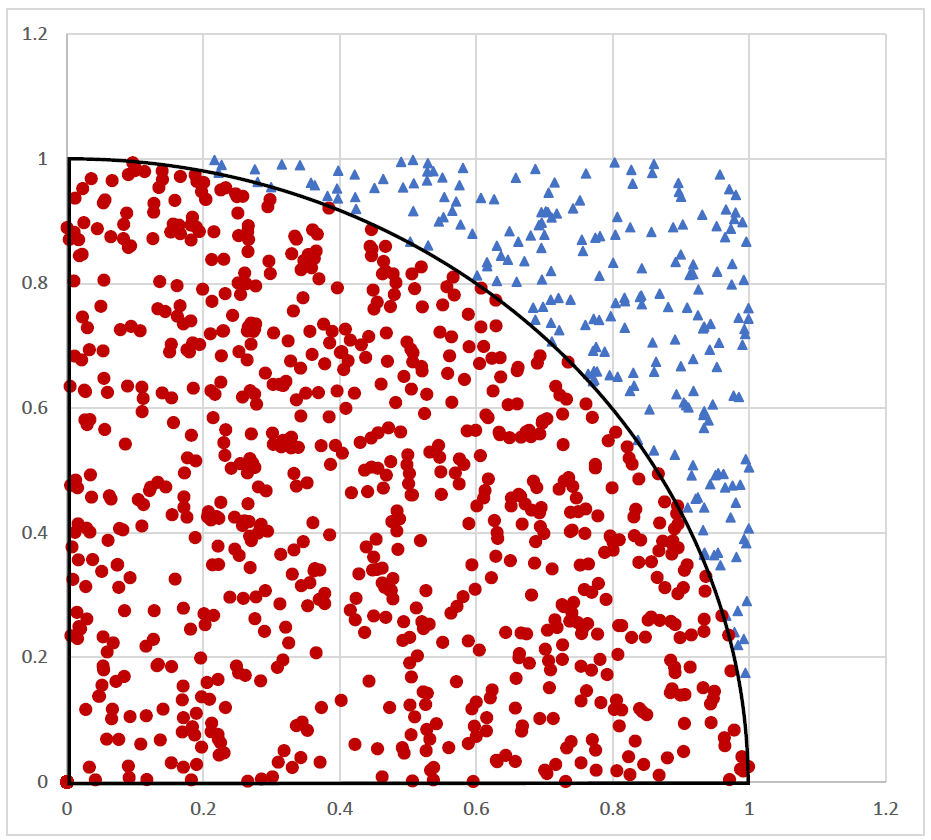
\includegraphics[scale=0.4]{images/monte-carlo-pi}\protect\caption{\label{fig:applications-Monte-Carlo-Pi}Ilustracja obliczania przybliżenia
liczby $\pi$ metodą Monte Carlo}
\end{figure}

\par\end{center}

Zwiększanie liczby próbek $n$ nie musi poprawiać dokładności otrzymanego
wyniku. W zależności od jakości zastosowanego generatora liczb pseudolosowych,
może on w pewnym momencie zakończyć bieżącą sekwencję i rozpocząć
zwracanie liczb z tej samej sekwencji od początku. Ponieważ celem
tego testu nie jest zbadanie dokładności przybliżenia liczby $\pi$
a porównanie szybkości obliczeń w klastrze i na pojedynczym węźle,
jako generator została wybrana klasa \dcscode{System.Random}%
\footnote{%
\begin{minipage}[t]{1\columnwidth}%
Implementacja klasy \dcscode{System.Random} w .NET Framework 4.0
posiada kilka cech, które sprawiają, że nie nadaje się ona do zastosowań,
w których oczekujemy ciągu o wysokim stopniu losowości. 
\begin{itemize}
\item Inicjowanie generatora przez domyślny konstruktor używa aktualnego
czasu. Z tego powodu utworzenie wielu jego instancji w krótkim czasie,
np. w środowisku wielowątkowym, może prowadzić do otrzymania takich
samych sekwencji liczb. Co więcej, przestrzeń inicujująca generator
jest stosunkowo mała -- mając już $2^{16}$ instancji generatora zainicjowanego
losowymi wartościami istnieje duże prawdopodobieństwo otrzymania tej
samej sekwencji wielokrotnie.
\item Dla niektórych wartości parametrów metoda \dcscode{Next} zwraca sekwencje,
których rozkład nie jest równomierny. 
\end{itemize}
W zastosowaniach, w których wymagane jest bezpieczeństwo zaleca się
stosowanie implementacji opartych o metody kryptograficzne, np. \dcscode{System.Security.Cryptography.RNGCryptoServiceProvider}.%
\end{minipage}%
}.

Otrzymane wyniki i ich analiza zostały przedstawione w rozdziale \dcsemph{Testy wydajnościowe i jakościowe}
w punkcie \ref{sub:performance-Obliczanie-przyblizenia-Pi}.


\chapter{Testy jakościowe i wydajnościowe}

W bibliotekach wykorzystywanych przez programistów równie ważna jak
bogata funkcjonalność czy łatwość użycia jest stabilność działania
i pewność, że błąd w~wykonaniu aplikacji nie leży po stronie biblioteki.
W związku z tym istotne jest pokrycie kodu biblioteki zestawem testów
zarówno jednostkowych jak i akceptacyjnych, które zostały opisane
w niniejszym rozdziale.

Oprócz testów jakościowych przeprowadzone zostały testy wydajnościowe,
które pozwoliły określić wydajność biblioteki w obecnym stanie implementacyjnym
oraz określić wpływ rodzaju przetwarzania na zasadność prowadzenia
przetwarzania rozproszonego.


\section{Testy jakościowe}

\label{sec:Testy-jako=00015Bciowe}Testy jakościowe pozwalają na sprawdzenie
konkretnych funkcji biblioteki w spreparowanym środowisku testowym.
Testy jednostkowe i integracyjne, działają w środowisku Microsoft
Unit Test Framework \cite{Microsoft-Unit-Test-Framework-for-Managed-Code}
zintegrowanym ze środowiskiem Visual Studio. Dodatkowo wykorzystana
została biblioteka Shoudly \cite{Shouldly} do zapisu asercji oraz
Moq \cite{Moq} do tworzenia atrap obiektów.


\subsection{Testy jednostkowe}

Testując niektóre funkcje biblioteki wskazane było sprawdzenie ich
zachowania abstrahując od ich zależności. W tym celu równolegle z
tworzonym kodem powstawały testy jednostkowe. Należy również zwrócić
uwagę, że testy jednostkowe wykonują się znacznie szybciej od testów
integracyjnych, co pozwala znacząco skrócić czas wykrycia oraz poprawy
ewentualnych błędów. Poniżej przedstawiono przykładowe przypadki testowe:
\begin{itemize}
\item \dcsname{lokalny wykonawca} -- operacja \dcscode{Join} z określonym
limitem czasu oczekiwania na jej zakończenie,
\item \dcsname{zdalny wykonawca} -- testy operacji \dcscode{Pulse} z użyciem
atrapy obiektu (ang.~\dcsemph{mock object}),
\item usługa \dcsname{zdalnego wykonawcy} -- wykonanie metody z użyciem
zserializowanego uchwytu, przechwytywanie wyjątków w kodzie użytkownika,
zwracanie statystyk obciążenia węzła oraz testy z użyciem zmienionej
implementacji interfejsu (ang.~\dcsemph{fake object}) -- operacji
\dcscode{Join} (synchronicznej i asynchronicznej), rzucenia przechwyconego
w kodzie użytkownika wyjątku w momencie wykonywania operacji \dcscode{Join},
wstrzykiwania zależności \dcscode{IBluepathCommunicationFramework}
(przez podmianę oraz przez dodanie brakującego parametru),
\item \dcsname{wątek rozproszony} -- wykonanie z użyciem \dcsname{lokalnego wykonawcy},
\dcsname{zdalnego wykonawcy} (potrzebne usługi, tj. \dcscode{IRemoteExecutorService}
i \dcscode{IScheduler} zostały zasymulowane za pomocą atrap obiektów,
użyto też \dcsname{zarządcy połączeń} w trybie bez wywołań zwrotnych),
głębokie kopiowanie parametrów wywołania,
\item planista \dcscode{ThreadNumberScheduler} -- test sprawdza, czy następuje
wybór najmniej obciążonego węzła spośród zasymulowanych,
\item z uwagi na użycie własnej klasy \dcscode{ServiceUri} jako klucza
w słowniku, testowano też taki scenariusz.
\end{itemize}

\subsection{Testy integracyjne}

W celu przetestowania działania funkcji takich jak przesyłanie klas
jako parametrów wskazane jest stworzenie testów integracyjnych. Ich
zadaniem jest przetestowanie nie tylko logiki wykonywanego kodu, ale
również wykrycie problemów jakie mogą się pojawić w związku z działaniem
w środowisku sieciowym (np. wymagane uprawnienia do utworzenia usługi
nasłuchującej, serializacja obiektów).

Jednym z problemów związanych z testami integracyjnymi jest potrzeba
stworzenia środowiska testowego. W momencie gdy zachodzi potrzeba
uruchomienia zewnętrznego programu (np. Redisa) system operacyjny
nie dostarcza narzędzi, które pozwoliłyby określić nie tylko czy dany
proces jest już uruchomiony, ale również czy skończył on proces inicjalizacji.
Należy również zwrócić uwagę, że testy nie powinny być od siebie zależne
-- a więc efekt wykonania jednego testu nie powinien mieć wpływu na
inne testy. Aby tego uniknąć, każdy test został wyposażony w taki
zestaw parametrów, który pozwoli mu się wykonać niezależnie od innych
(np. port na którym ma nasłuchiwać usługa \dcsname{Bluepath}).

W ramach testów integracyjnych przetestowane zostały następujące aspekty:
\begin{itemize}
\item \dcsname{wątki rozproszone} -- zachowanie systemu w wyniku próby
wykonania metod akceptujących różne typy parametrów i zwracające wyniki
różnego typu -- tablice, klasy (także generyczne), delegaty, a także
obsługa wyjątków w kodzie użytkownika oraz w przypadku nieprawidłowego
wywołania; test obejmował także wykonanie metody z biblioteki napisanej
w języku F\#,
\item \dcsname{zarządca połączeń} -- pobieranie listy dostępnych węzłów
z \dcsname{usługi odnajdywania węzłów} i aktualizowanie swojej
lokalnej kopii listy (dodawanie nowych węzłów i usuwanie wyrejestrowanych),
pobieranie informacji o obciążeniu węzłów zarejestrowanych w klastrze,
\item \dcsname{pamięć rozproszona} -- testy zapisu i odczytu obiektów
(także jako operacji zbiorczych),
\item \dcsname{zamki rozproszone} -- pobieranie i zwalnianie zamków (także
z limitem czasu), budzenie wątków czekających na zamkach,
\item a także testy struktur danych i obiektów zbudowanych na bazie \dcsname{pamięci rozproszonej}
-- lista, słownik, licznik.
\end{itemize}

\section{Testy wydajnościowe}

Ważną częścią tworzenia biblioteki programistycznej jest zweryfikowanie
jej zachowania w przykładowych zastosowaniach. Pozwala to zweryfikować
słuszność przyjętych założeń i rozwiązań. 

Przy okazji weryfikacji działania biblioteki \dcsname{Bluepath} przeprowadzone
zostały testy wydajnościowe, zestawiające efekt wykonania przetwarzania
w klastrze w stosunku do przetwarzania na pojedynczym procesorze oraz
porównanie dostarczonych przykładowych algorytmów szeregowania zadań.


\subsection{Środowisko }

Środowisko do przeprowadzenia testów wydajnościowych zostało przygotowane
w~oparciu o platformę Microsoft Azure \cite{Microsoft-Azure}. Klaster
składał się z 7 maszyn wirtualnych -- na sześciu z nich działały usługi
systemu Bluepath pod kontrolą systemu operacyjnego Windows Server
2012 R2 Datacenter (wydanego 17 czerwca 2014 r.), a na jednej maszynie
uruchomiony został host \dcsname{pamięci rozproszonej} Redis pod
kontrolą systemu operacyjnego Ubuntu Server 14.04 LTS (wydanego 20
czerwca 2014 r.). Maszyny różniły się konfiguracją sprzętową w zależności
od przeznaczenia:
\begin{itemize}
\item węzeł inicjujący przetwarzanie był typu \dcsname{Medium VM (Basic A2)}
i posiadał 2~wirtualne rdzenie AMD Operton 1,6 GHz i 3,5 GB pamięci
operacyjnej, 
\item węzły obliczeniowe były typu \dcsname{Small VM (Basic A1)} dysponowały
po 1 wirtualnym rdzeniu AMD Opteron 1,6 GHz i 1,75 GB pamięci operacyjnej, 
\item węzeł hostujący usługę Redis była to instancja typu \dcsname{Large VM (Basic A3)}
posiadająca cztery rdzenie AMD Opteron 1,6 GHZ i 7 GB pamięci operacyjnej. 
\end{itemize}
Szczegóły konfiguracji zestawiono w tabeli \ref{tab:performance-Konfiguracja-testowego-klastra}.
Maszyny wirtualne wchodzące w~skład klastra połączone zostały w wirtualną
sieć, w której wyłączone były zapory sieciowe, a komunikacja odbywała
się z użyciem prywatnych wewnętrznych adresów IP (tzw. \dcsname{DIP},
przydzielony automatycznie przez Windows Azure z użyciem DHCP). 

\begin{table}
\centering{}\protect\caption{\label{tab:performance-Konfiguracja-testowego-klastra}Konfiguracja
testowego klastra}
\begin{tabular}{|c|c|c|c|c|}
\hline 
Nazwa maszyny & Typ instancji & Liczba rdzeni & Pamięć RAM & System operacyjny\tabularnewline
\hline 
\hline 
Master & A2 & 2 & 3,5 GB & Windows Server\tabularnewline
\hline 
Slave1 & A1 & 1 & 1,75 GB & Windows Server\tabularnewline
\hline 
Slave2 & A1 & 1 & 1,75 GB & Windows Server\tabularnewline
\hline 
Slave3 & A1 & 1 & 1,75 GB & Windows Server\tabularnewline
\hline 
Slave4 & A1 & 1 & 1,75 GB & Windows Server\tabularnewline
\hline 
Slave5 & A1 & 1 & 1,75 GB & Windows Server\tabularnewline
\hline 
Redis & A3 & 4 & 7 GB & Ubuntu Server\tabularnewline
\hline 
\end{tabular}
\end{table}


Do dystrybucji nowych wersji bibliotek systemu Bluepath na wszystkie
maszyny w klastrze przygotowany został skrypt PowerShell przedstawiony
na listingu \ref{lis:performance-Skrypt-dystrybuuj=000105cy-biblioteki}.
Wykorzystuje on opisany w punkcie \ref{sec:implementation-Skrypt-Send-Folder}
skrypt \dcspath{Send-Folder}.

\inputencoding{latin2}\begin{lstlisting}[caption={Skrypt
dystrybuuj±cy biblioteki w klastrze},label={lis:performance-Skrypt-dystrybuuj=000105cy-biblioteki},breaklines=true,language=bash,numbers=left]
.\Send-Folder.ps1 -server [adres wêz³a 1] -user [nazwa u¿ytkownika] 
  -password [has³o] -source [folder ¼ród³owy] -destination [folder docelowy]
...
.\Send-Folder.ps1 -server [adres wêz³a n] -user [nazwa u¿ytkownika] 
  -password [has³o] -source [folder ¼ród³owy] -destination [folder docelowy]
\end{lstlisting}
\inputencoding{utf8}


\subsection{Generowanie słownika prefiksów}

Jednym z algorytmów wykorzystanych do pomiaru wydajności był algorytm
tworzący prefiksy na potrzeby przeprowadzenia operacji uzupełniania
tekstu opisany w~punkcie \ref{sub:zastosowania-autocomplete-Wczytywanie-danych}.
Dla określonej liczby dokumentów znajdujących się w \dcsname{pamięci rozproszonej}
pomiar czasu przetwarzania był powtarzany dziesięć razy. Wykres \ref{fig:performance-Generowanie-prefixow}
przedstawia porównanie uśrednionych czasów generowania słownika prefiksów
na pojedynczym węźle oraz w klastrze. Dla zbioru 10000 dokumentów
udało się uzyskać prawie dwukrotne przyspieszenie w stosunku do przetwarzania
na pojedynczej maszynie. Warto również nadmienić, że w algorytmie
testującym wprowadzono mechanizm okresowo czyszczący lokalną pamięć
prefiksów ze względu na wyczerpywanie się pamięci w przypadku przetwarzania
na pojedynczym węźle.

\begin{figure}
\centering{}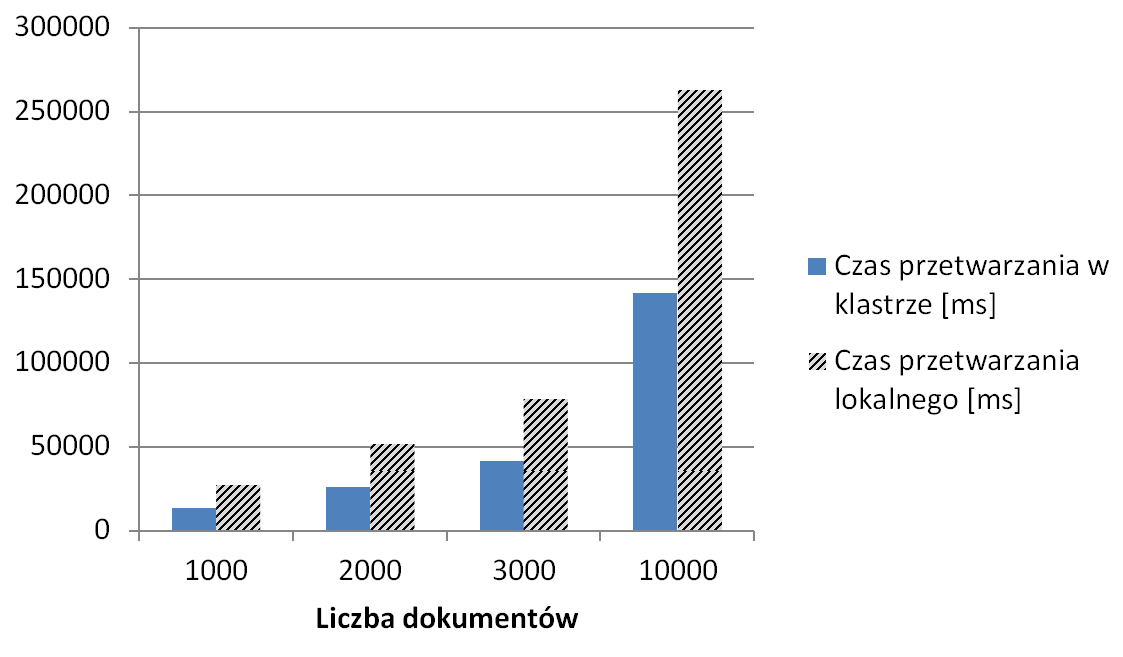
\includegraphics[scale=0.5]{images/prefixy-6}\protect\caption{\label{fig:performance-Generowanie-prefixow}Porównanie czasu generowania
słownika prefiksów }
\end{figure}



\subsection{Obliczanie przybliżenia liczby $\pi$}

\label{sub:performance-Obliczanie-przyblizenia-Pi}Kolejnym algorytmem,
przy pomocy którego zmierzono zysk związany z zastosowaniem biblioteki
Bluepath było obliczanie przybliżenia liczby $\pi$ metodą przedstawioną
w punkcie \ref{sec:Przykladowe-zastosowania-liczba-pi}. Wykres \ref{fig:performace-Por=0000F3wnanie-czasu-obliczania-pi}
przedstawia porównanie uśrednionych czasów przetwarzania na pojedynczym
węźle oraz w klastrze w zależności od rozmiaru instancji. Czas został
przedstawiony w skali logarytmicznej. 

\begin{figure}
\centering{}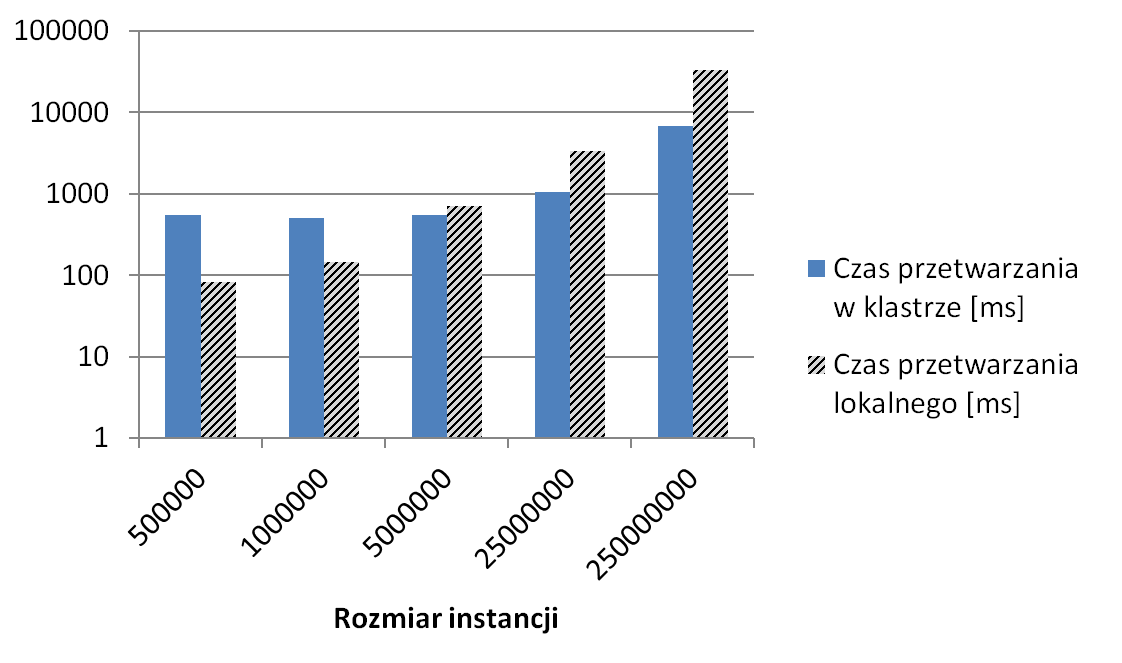
\includegraphics[scale=0.5]{images/pi-5-machines}\protect\caption{\label{fig:performace-Por=0000F3wnanie-czasu-obliczania-pi}Porównanie
czasu obliczania przybliżenia liczby $\pi$}
\end{figure}


Dla dużych instancji przetwarzanie przy pomocy biblioteki Bluepath
jest dużo szybsze niż przetwarzanie na pojedynczym węźle. Jednak dla
małych instancji narzut generowany przez bibliotekę sprawia, że przetwarzanie
w klastrze staje się mniej efektywne niż przetwarzanie lokalne. Można
to również zauważyć na wykresie \ref{fig:performace-Przyspieszenie-pi}.
Przedstawia on przyspieszenie uzyskane w związku z zastosowaniem biblioteki
Bluepath do przetwarzania w klastrze w stosunku do przetwarzania na
pojedynczym węźle. 

\begin{figure}
\centering{}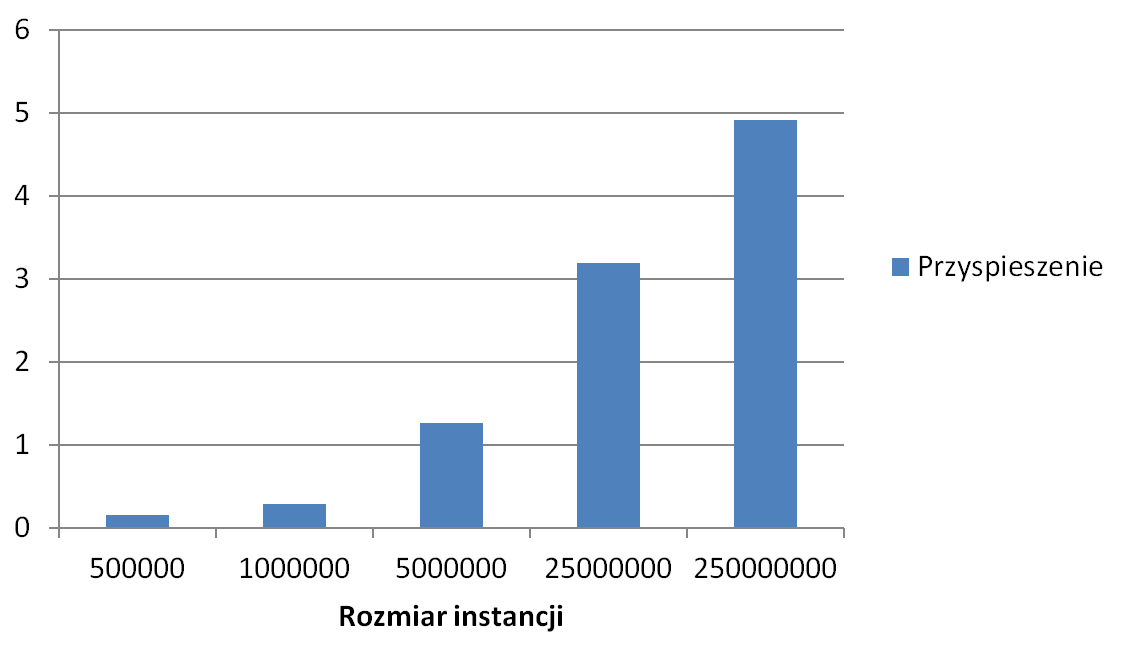
\includegraphics[scale=0.5]{images/pi-5-speedup}\protect\caption{\label{fig:performace-Przyspieszenie-pi}Przyspieszenie w stosunku
do przetwarzania lokalnego}
\end{figure}


Narzut widoczny na obu wykresach jest częstym zjawiskiem w systemach
rozproszonych i wynika z konieczności przeprowadzenia komunikacji
sieciowej.


\chapter{Podsumowanie}

Niniejszy rozdział stanowi podsumowanie pracy. Omówiono w nim przebieg
realizacji, napotkane w trakcie implementacji problemy oraz przedstawiono
potencjalne kierunki dalszego rozwoju projektu.


\section{Przebieg realizacji}

W trakcie realizacji tej pracy udało się zrealizować główny cel --
zaprojektowanie biblioteki wspomagającej użytkowników w implementacji
aplikacji rozproszonych (por. punkt \ref{sec:intro-cel-i-zakres}).
Wszystkie przyjęte założenia były weryfikowane poprzez implementację
prototypu opisaną w rozdziale \ref{chap:implementation}. W obecnym
momencie biblioteka posiada zależność jedynie od usługi Redis wykorzystywanej
do realizacji \dcsname{pamięci rozproszonej}. Należy jednak nadmienić,
że zależność tę można w łatwy sposób usunąć poprzez dostarczenie własnej
implementacji \dcsname{pamięci rozproszonej} co jest możliwe dzięki
modułowości biblioteki.

Biblioteka i założenia poczynione przy jej tworzeniu zostały dodatkowo
zweryfikowane poprzez implementację aplikacji opisanych w rozdziale
\ref{chap:applications}. Możliwość wykorzystania \dcsemph{debuggera}
w trakcie tworzenia tych aplikacji oraz testowania działania biblioteki
okazała się niezastąpiona i stanowiła duży atut.




\section{Napotkane problemy}

W trakcie realizacji pracy napotkano problemy, których opis i rozwiązania
opisano poniżej. Ich natura była bardzo różna, wynikały głównie z
błędów i ograniczeń w~wykorzystywanym kodzie pochodzącym od innych
twórców:
\begin{itemize}
\item serializacja wyjątków,
\item niezaimplementowane do końca wewnętrzne metody w Rhino DHT,
\item ograniczenie wydajności środowiska Redis w wyniku przenoszenia kodu
z systemu Linux do systemu Windows,
\item błędy składniowe w plikach XML Schema Definition pochodzących z bibliteki
OpenXES.
\end{itemize}

\subsection{Serializacja}

Wszystkie wyjątki w .NET Framework powinny być serializowalne. Okazuje
się jednak, że klasa bazowa \dcscode{Exception} zawiera wirtualne
pole \dcscode{Data} typu \dcscode{IDictionary}, które umożliwia
dodanie do kolekcji obiektu, który nie będzie serializowalny. Pomimo
tego, że każdy wstawiany obiekt jest sprawdzany pod tym kątem poprzez
sprawdzenie flagi \dcscode{Type.IsSerializable}, nie gwarantuje to,
że jego składowe będą serializowalne, a tym samym i cały wyjątek. 

Drugim problemem jest zachowanie klasy \dcscode{DataContractSerializer}.
Zakładając, że definicja wiadomości (\dcscode{DataContract}) zawiera
pole typu \dcscode{Exception}, w którym ma zostać przesłany wyjątek,
\dcscode{DataContractSerializer} wymaga dodania atrybutu \dcscode{KnownType}
dla każdego typu wyjątku wywiedzionego z typu \dcscode{Exception},
który ma zostać przesłany na zdalną stronę, również tego zawartego
w polu na wyjątek wewnętrzny (\dcscode{InnerException)}. Dodawanie
atrybutu \dcscode{KnownType} dla każdego typu wyjątku, który może
zostać wygenerowany przez kod użytkownika jest rozwiązaniem dalekim
od transparentnego, w związku z tym zdecydowano o przesyłaniu wyjątków
w formie tekstowej -- wywoływana jest na nich rekurencyjnie metoda
\dcscode{ToString}.


\subsection{Rhino DHT}

\label{par:problemy-rhino-dht}W punkcie \ref{sub:implementation-Pamiec-rozproszona-rozwazane-rozwiazania},
gdzie opisano wybór aplikacji do zrealizowania \dcsname{pamięci rozproszonej},
zasygnalizowano problem, który był powodem porzucenia biblioteki Rhino
DHT. Zgodnie z założeniami przedstawionymi w punkcie \ref{def:concept-Pamiec-rozproszona},
biblioteka powinna udostępniać mechanizmy atomowego porównania i zapisu
bądź atomowego odczytu i zapisu. Przykładowa implementacja \dcsname{zamka rozproszonego}
miała opierać się o mechanizm wersjonowania danych obecny w Rhino
DHT:
\begin{itemize}
\item pobranie aktualnej, najnowszej wersji pola reprezentującego wartość
zamka (wolny/zajęty przez wykonawcę o danym \dcscode{eid}) wraz z
numerem wersji \dcsemph{k},
\item w przypadku gdy zamek jest wolny -- zapis nowej wersji wartości pola
(własnego identyfikatora \dcscode{eid}) ze wskazaniem wersji \dcsemph{k}
jako rodzica,
\item odczyt wersji \dcsemph{k+1} i porównanie z własnym eid -- jeżeli
jest równe oznacza to, że zamek został pobrany, w przeciwnym wypadku
-- że został zajęty przez inny proces,
\item zwolnienie zamka odbywać się miała poprzez zapis odpowiedniej informacji
ze wskazaniem wersji \dcsemph{k+1} jako rodzica.
\end{itemize}
Widać zatem, że zapisy miały tworzyć strukturę drzewiastą, gdzie najdłuższa
ścieżka miała reprezentować sekwencję pobranych i zwolnionych zamków.
Niestety wewnętrznie nie wszystkie operacje zostały zaimplementowane,
co objawiało się wyjątkiem \dcscode{NotImplementedException} zgłaszanym
z wewnątrz biblioteki Rhino DHT.


\subsection{Redis uruchamiany w systemie Windows}

\label{par:problemy-Windows-Redis}Podczas pracy usługi Redis z dużym
obciążeniem pod kontrolą systemu Windows zaobserwowano znaczący spadek
wydajności. Wyjaśnienie problemów z działaniem znaleziono w dokumencie
\cite{MSOpenTech-Redis-Release-Notes}. 

W wersji dla systemu Linux wszystkie operacje wejścia-wyjścia korzystają
z deskryptorów plików, które nie są tak rozpowszechnione w API systemu
Windows. Wersja przeznaczona dla systemów Windows używa w związku
z tym symulowanego deskryptora plików. Zasadniczym problemem jest
jednak brak obecności wywołania systemowego \dcscode{fork} do tworzenia
procesów potomnych, która w systemie Windows została zasymulowana
poprzez umieszczenie sterty procesu Redis w \dcsemph{memory-mapped file},
czyli fragmencie pamięci wirtualnej, która jest dokładnym odwzorowaniem
pliku znajdującego się na dysku lub -- w ogólności -- obiektu, do
którego jesteśmy w stanie uzyskać deskryptor. Taki deskryptor przekazywany
jest następnie potomnym procesom. Warto zauważyć, że domyślnym zachowaniem
środowiska jest tworzenie współdzielonego pliku o rozmiarze odpowiadającym
rozmiarowi pamięci fizycznej komputera. 

Ostatecznie różnice, które ujawniły się pomiędzy wersją usługi Redis
przeznaczoną dla systemów Windows a pochodnych UNIXa, wpłynęły na
podjęcie decyzji o uruchomieniu go w systemie operacyjnym Ubuntu.


\subsection{Implementacja standardu OpenXES}

\label{sub:problemy-Implementacja-standardu-OpenXES-z-XSD}Podczas
próby implementacji standardu OpenXES opisanej w punkcie \ref{sec:implementation-Logowanie-zdarzen}
na podstawie plików XML Schema udostępnionych 28 marca 2014 r. wraz
z wersją 2.0 bibliteki napotkano problemy przy próbie automatycznego
wygenerowania klas. W~jednym z plików, \dcscode{xes.xsd}, znaleziony
został drobny błąd składniowy -- brakująca spacja, co powodowało,
że plik XML był niepoprawny składniowo i nieprzyjmowany przez narzędzie
\dcscode{xsd.exe}. Po jego poprawieniu ujawnił się kolejny problem
objawiający się wyjątkiem przepełnienia stosu w trakcie generowania
klas. Ten problem został rozwiązany przez objęcie wnętrza elementu
\dcscode{xs:complexType} odnoszącego się do typu \dcscode{AttributableType}
elementem \dcscode{xs:sequence}.


\section{Perspektywy dalszego rozwoju}

Przy projektowaniu biblioteki Bluepath został zdefiniowany szereg
założeń oraz podjęto szereg decyzji projektowych przedstawionych w
rozdziałach trzecim i czwartym. Poniżej wskazano potencjalne kierunki
rozwoju projektu -- rozluźniania pewnych założeń i rozbudowy funkcjonalności.


\subsection{Niezawodność przetwarzania}

\label{sub:conclusions-Obsluga-awarii}Aspektem, który nie został
poruszony w niniejszej pracy jest zapewnienie niezawodności przetwarzania
w przypadku awarii węzłów (por. punkt \ref{sec:concept-Obsluga-awarii}).
Poniżej zaproponowano sposoby obsługi awarii różnych komponentów --
mogą one dotyczyć węzłów danych, węzłów obliczeniowych a także \dcsname{usługi odnajdywania węzłów}.


\subsubsection*{Obsługa awarii węzłów danych}

Zapewnienie bezpieczeństwa węzłów danych leży po stronie wybranej
do ich zrealizowania aplikacji (por. punkt \ref{sec:concept-Rozproszona-pami=000119=000107-wsp=0000F3=000142dzielona}).
Wykorzystywany obecnie system Redis może zostać uruchomiony w trybie
z replikacją, w którym jeden z węzłów jest punktem dostępowym do zapisu
lub odczytu, a jego repliki udostępniają dane tylko do odczytu. Po
awarii węzła nadrzędnego jedna z replik staje się nowym punktem dostępowym
z możliwością zapisu.

Istnieje również wariant systemu -- Redis Cluster -- w którym dane
dzielone są pomiędzy węzły, udostępniający mechanizmy replikacji i
rekonfiguracji w przypadku awarii.


\subsubsection*{Obsługa awarii węzłów obliczeniowych}

W przypadku, gdy aplikacja nie posiada współdzielonego stanu, czyli
nie wykorzystuje rozproszonych struktur danych ani obiektów -- a więc
wywołania są idempotentne -- obsługa awarii węzłów obliczeniowych
mogłaby uwzględniać drzewiasty charakter takiego przetwarzania. \dcsname{Wątki rozproszone}
zainicjowane przez stracony węzeł musiałyby być wycofane, a węzeł
nadrzędny musiałby zlecić jeszcze raz wykonanie przerwanego wątku.
\dcsname{Wątki rozproszone}, które mogą być bezpiecznie uruchamiane
ponownie musiałyby być \dcsemph{explicite} oznaczane przez programistę
flagą (\dcscode{Resumable}) lub z wykorzystaniem dedykowanej metody
(\dcscode{AsResumable}). 


\subsubsection*{Obsługa awarii serwera usługi odnajdywania węzłów}

Wrażliwym punktem jest również scentralizowany serwer \dcsname{usługi odnajdywania węzłów}.
Warto jednak zauważyć, że prawdopodobieństwo awarii jednego konkretnego
węzła jest dużo niższe niż prawdopodobieństwo awarii dowolnego węzła
w klastrze. Argumentem, który przemawia za koniecznością zajęcia się
tym problemem jest kluczowe znaczenie serwera \dcsname{usługi odnajdywania węzłów}
do realizacji przetwarzania. Aby zapewnić niezawodność dostępu do
\dcsname{usługi odnajdywania węzłów} możnaby uruchomić jego replikę,
która przejęłaby zadania po awarii podstawowego serwera (podejście
to wykorzystywane jest np. w MapReduce, gdzie \dcsemph{name node}
jest replikowany). Warto również rozważyć implementację opartą o rozproszoną
tablcę haszową (ang.~\dcsemph{distributed hash table}, DHT) z replikacją.


\subsection{Rozbudowa funkcjonalności}

Ponieważ z przetwarzaniem rozproszonym wiąże się wiele problemów,
a przy tworzeniu biblioteki zauważano kolejne obszary w których możnaby
zmniejszyć nakład pracy użytkownika nie było możliwe zrealizowanie
wszystkich funkcji. Poniżej przedstawiono przykładowe obszary, w których
możnaby rozbudować funkcjonalność systemu:
\begin{itemize}
\item rozproszone struktury danych -- np. implementacja kolejki,
\item interfejs do komunikacji z systemem -- rozbudowa o metody dostępu
do pamięci lokalnej węzła (\dcscode{LocalStorage}), dodanie możliwości
raportowania zaawansowania przetwarzania w ramach wątku (\dcscode{ReportProgress})
w celu budowy dokładniejszych planistów,
\item DLINQ -- implementacja pozostałych metod obecnych w standardowym LINQ
i niedostępnych w obecnej implementacji,
\item wykorzystanie asynchronicznych wzorców z .NET Framework 4.5 (\dcscode{async},
\dcscode{await}) -- obecnie jedyną operacją asynchroniczną jest oczekiwanie
na zakończenie \dcsname{wątku rozproszonego} -- \dcscode{JoinAsync}.
\end{itemize}

\section{Zakończenie}

W niniejszej pracy przeanalizowano i porównano istniejące rozwiązania
wspomagające programistów w tworzeniu aplikacji rozproszonych oraz
zaprojektowano i zaimplementowano prototyp biblioteki, która pozwala
jej użytkownikom w prosty sposób zaimplementować program przetwarzający
dane w sposób rozproszony. Użytkownik pisząc program w sposób podobny
do tego, w jaki pisałby program równoległy, uzyskuje program wykorzystujący
moc obliczeniową wielu węzłów w klastrze. W takim przypadku wątki,
zamiast wykonywać się na wielu rdzeniach jednego procesora, wykonują
się na zdalnych maszynach. Prototyp biblioteki został przetestowany
zarówno pod względem jakościowym jak i wydajnościowym. Przedstawiono
również przykładowe zastosowania biblioteki. Biorąc powyższe pod uwagę
można uznać, że wszystkie założone cele pracy zostały zrealizowane.

\backmatter

\nocite{*}
\begin{thebibliography}{10}

\bibitem{ArpaciDusseau14-Book}
R.~H. Arpaci-Dusseau i A.~C. Arpaci-Dusseau.
\newblock {\em {Operating Systems: Three Easy Pieces}}.
\newblock Arpaci-Dusseau Books, Maj 2014.

\bibitem{DSM}
K.~Li i P.~Hudak.
\newblock {Memory Coherence in Shared Virtual Memory Systems}, Listopad 1989.
\newblock ACM TOCS, 7:4.

\bibitem{RPC}
A.~D. Birrell i B.~J. Nelson.
\newblock {Implementing Remote Procedure Calls}, Luty 1984.
\newblock ACM TOCS, Volume 2:1.

\bibitem{Misra83}
J.~Misra.
\newblock {Detecting Termination of Distributed Computations Using Markers}.
\newblock W {\em {Proceedings of the $2^{nd}$ annual ACM Symposium on
  Principles of Distributed Computing (PODC)}}, Montreal, Canada, 1983.

\bibitem{Dijkstra-Diffusing}
E.~W. Dijkstra i C.~S. Scholten.
\newblock {Termination Detection for Diffusing Computations}.
\newblock 1980.

\bibitem{PVM}
A.~Geist, A.~Beguelin, J.~Dongarra, W.~Jiang, R.~Manchek  i V.~Sunderam.
\newblock {\em {PVM: Parallel Virtual Machine A Users' Guide and Tutorial for
  Networked Parallel Computing}}.
\newblock MIT Press, 1994.
\newblock \url{http://www.netlib.org/pvm3/book/pvm-book.html}.

\bibitem{MPI-Standard-Version-3}
{MPI: A Message-Passing Interface Standard}.
\newblock \url{http://www.mpi-forum.org/docs/mpi-3.0/mpi30-report.pdf}.

\bibitem{Using-MPI-Portable-Parallel-Programming-with-the-Message-Passing-Interface}
W.~Gropp, E.~Lusk  i A.~Skjellum.
\newblock {\em {Using MPI: Portable Parallel Programming with the
  Message-Passing Interface}}.
\newblock MIT Press, Cambridge, MA, USA, 1999.

\bibitem{Microsoft-Research-Dryad}
{Microsoft Research -- Dryad}.
\newblock \url{http://research.microsoft.com/en-us/projects/dryad/}.

\bibitem{SCOPE}
R.~Chaiken, B.~Jenkins, P.~Åke Larson, B.~Ramsey, D.~Shakib, S.~Weaver  i
  J.~Zhou.
\newblock {SCOPE: Easy and Efficient Parallel Processing of Massive Data Sets}.
\newblock
  \url{http://research.microsoft.com/en-us/um/people/jrzhou/pub/Scope.pdf}.

\bibitem{SQL}
IBM.
\newblock {\em {IBM® DB2® Universal Database SQL Reference}}.
\newblock 2001.
\newblock
  \url{ftp://ftp.software.ibm.com/ps/products/db2/info/vr7/pdf/letter/db2s0e71.pdf}.

\bibitem{DryadLINQ-MSR}
Y.~Yu, M.~Isard, D.~Fetterly, M.~Budiu, U.~Erlingsson, P.~K. Gunda  i
  J.~Currey.
\newblock {DryadLINQ: A System for General-Purpose Distributed Data-Parallel
  Computing Using a High-Level Language}.
\newblock Symposium on Operating System Design and Implementation (OSDI), San
  Diego, CA, USA, Grudzień 2008.
\newblock \url{http://research.microsoft.com/projects/dryadlinq/}.

\bibitem{DryadLINQ-discarded}
D.~Pattee.
\newblock {Announcing the Windows Azure HPC Scheduler and HPC Pack 2008 R2
  Service Pack 3 releases}.
\newblock
  \url{http://blogs.technet.com/b/windowshpc/archive/2011/11/11/hpc-pack-2008-r2-sp3-and-windows-azure-hpc-scheduler-released.aspx}.

\bibitem{Google-MapReduce}
J.~Dean i S.~Ghemawat.
\newblock {MapReduce: Simplified Data Processing on Large Clusters}.
\newblock Sixth Symposium on Operating System Design and Implementation (OSDI),
  San Francisco, CA, USA, Grudzień 2004.
\newblock \url{http://research.google.com/archive/mapreduce.html}.

\bibitem{HDFS-Architecture-Guide}
D.~Borthakur.
\newblock {HDFS Architecture Guide}.
\newblock \url{http://hadoop.apache.org/docs/r1.1.2/hdfs_design.html}.

\bibitem{Spark-Berkeley}
M.~Zaharia, M.~Chowdhury, M.~J. Franklin, S.~Shenker  i I.~Stoica.
\newblock {Spark: Cluster Computing with Working Sets}.
\newblock \url{http://spark.apache.org/research.html}.

\bibitem{Spark-Berkeley-Performance}
R.~S. Xin, M.~Z. Josh~Rosen, M.~J. Franklin, S.~Shenker  i I.~Stoica.
\newblock {Shark: SQL and Rich Analytics at Scale}.
\newblock
  \url{https://amplab.cs.berkeley.edu/wp-content/uploads/2013/02/shark_sigmod2013.pdf}.

\bibitem{Erlang-Armstrong:2010:ERL:1810891.1810910}
J.~Armstrong.
\newblock Erlang.
\newblock {\em Communications of the ACM}, 53(9):68--75, Wrzesień 2010.
\newblock \url{http://doi.acm.org/10.1145/1810891.1810910}.

\bibitem{Orleans-export:210931}
P.~A. Bernstein, S.~Bykov, A.~Geller, G.~Kliot  i J.~Thelin.
\newblock Orleans: Distributed virtual actors for programmability and
  scalability.
\newblock Raport techniczny MSR-TR-2014-41, Marzec 2014.
\newblock \url{http://research.microsoft.com/apps/pubs/default.aspx?id=210931}.

\bibitem{Hadoop-Python}
M.~G. Noll.
\newblock {Writing an Hadoop MapReduce Program in Python}.
\newblock
  \url{http://www.michael-noll.com/tutorials/writing-an-hadoop-mapreduce-program-in-python/}.

\bibitem{MSDN:WhatIsWindowsCommunicationFoundation}
{MSDN -- What Is Windows Communication Foundation}.
\newblock \url{http://msdn.microsoft.com/en-us/library/ms731082.aspx}.

\bibitem{rfc1631}
K.~Egevang i P.~Francis.
\newblock {The IP Network Address Translator (NAT)}.
\newblock RFC 1631 (Informational), Maj 1994.
\newblock \url{http://www.ietf.org/rfc/rfc1631.txt}.
\newblock Obsoleted by RFC 3022.

\bibitem{rfc3022}
P.~Srisuresh i K.~Egevang.
\newblock {Traditional IP Network Address Translator (Traditional NAT)}.
\newblock RFC 3022 (Informational), Styczeń 2001.
\newblock \url{http://www.ietf.org/rfc/rfc3022.txt}.

\bibitem{Microsoft.NET}
{Microsoft .NET}.
\newblock \url{http://www.microsoft.com/net/}.

\bibitem{rfc675}
V.~Cerf, Y.~Dalal  i C.~Sunshine.
\newblock {Specification of Internet Transmission Control Program}.
\newblock RFC 675, Grudzień 1974.
\newblock \url{http://www.ietf.org/rfc/rfc675.txt}.

\bibitem{rfc793}
J.~Postel.
\newblock {Transmission Control Protocol}.
\newblock RFC 793 (INTERNET STANDARD), Wrzesień 1981.
\newblock \url{http://www.ietf.org/rfc/rfc793.txt}.
\newblock Updated by RFCs 1122, 3168, 6093, 6528.

\bibitem{rfc1122}
R.~Braden.
\newblock {Requirements for Internet Hosts - Communication Layers}.
\newblock RFC 1122 (INTERNET STANDARD), Październik 1989.
\newblock \url{http://www.ietf.org/rfc/rfc1122.txt}.
\newblock Updated by RFCs 1349, 4379, 5884, 6093, 6298, 6633, 6864.

\bibitem{rfc2616}
R.~Fielding, J.~Gettys, J.~Mogul, H.~Frystyk, L.~Masinter, P.~Leach  i
  T.~Berners-Lee.
\newblock {Hypertext Transfer Protocol -- HTTP/1.1}.
\newblock RFC 2616 (Draft Standard), Czerwiec 1999.
\newblock \url{http://www.ietf.org/rfc/rfc2616.txt}.
\newblock Obsoleted by RFCs 7230, 7231, 7232, 7233, 7234, 7235, updated by RFCs
  2817, 5785, 6266, 6585.

\bibitem{W3C-SOAP11}
D.~Box, D.~Ehnebuske, G.~Kakivaya, A.~Layman, N.~Mendelsohn, H.~F. Nielsen,
  S.~Thatte  i D.~Winer.
\newblock {Simple Object Access Protocol (SOAP) 1.1}.
\newblock Raport techniczny, W3C, Maj 2000.
\newblock http://www.w3.org/TR/2000/NOTE-SOAP-20000508/.

\bibitem{W3C-SOAP12-part0}
N.~Mitra i Y.~Lafon.
\newblock {SOAP Version 1.2 Part 0: Primer}.
\newblock druga wersja rekomendacji, W3C, Kwiecień 2007.
\newblock http://www.w3.org/TR/2007/REC-soap12-part0-20070427/.

\bibitem{W3C-SOAP12-part1}
M.~Gudgin, M.~Hadley, N.~Mendelsohn, J.-J. Moreau, H.~F. Nielsen, A.~Karmarkar
  i Y.~Lafon.
\newblock {SOAP Version 1.2 Part 1: Messaging Framework}.
\newblock druga wersja rekomendacji, W3C, Kwiecień 2007.
\newblock http://www.w3.org/TR/2007/REC-soap12-part1-20070427/.

\bibitem{Tannenbaum-SOP}
A.~S. Tannenbaum.
\newblock {\em {Systemy operacyjne}}, strony 204--205.
\newblock Helion, 2010.

\bibitem{Memcached}
{Strona projektu Memcached}.
\newblock \url{http://www.memcached.org/}.

\bibitem{Riak}
{Strona projektu Riak}.
\newblock \url{http://basho.com/riak/}.

\bibitem{Amazon-Dynamo}
G.~DeCandia, D.~Hastorun, M.~Jampani, G.~Kakulapati, A.~Lakshman, A.~Pilchin,
  S.~Sivasubramanian, P.~Vosshall  i W.~Vogels.
\newblock {Dynamo: Amazon’s Highly Available Key-value Store}.
\newblock ACM Symposium on Operating Systems Principles, Październik 2007.
\newblock
  \url{http://www.allthingsdistributed.com/files/amazon-dynamo-sosp2007.pdf}.

\bibitem{Polyphony-blog-1}
D.~Mohl.
\newblock {.NET Remoting in F\#: A Start to a Distributed Hash Table (DHT)}.
\newblock
  \url{http://bloggemdano.blogspot.com/2010/04/net-remoting-in-f-start-to-distributed.html}.

\bibitem{Polyphony-blog-2}
D.~Mohl.
\newblock {A Distributed Hash Table (DHT) in F\#: Moving from .NET Remoting to
  WCF}.
\newblock
  \url{http://bloggemdano.blogspot.com/2010/04/distributed-hash-table-dht-in-f-moving.html}.

\bibitem{Polyphony-blog-3}
D.~Mohl.
\newblock {A Distributed Hash Table (DHT) in F\#: Using Higher Order Functions
  for the Service Operation Calls}.
\newblock
  \url{http://bloggemdano.blogspot.com/2010/04/distributed-hash-table-dht-in-f-using.html}.

\bibitem{Polyphony-repo}
{Repozytorium kodu projektu Polyphony}.
\newblock \url{https://github.com/dmohl/Polyphony/}.

\bibitem{Rhino-DHT}
{Strona projektu Rhino DHT}.
\newblock \url{https://github.com/ayende/rhino-dht/}.

\bibitem{Rhino-PHT}
{Strona projektu Rhino PHT}.
\newblock \url{https://github.com/ayende/rhino-pht/}.

\bibitem{Rhino-Queues}
{Strona projektu Rhino Queues}.
\newblock \url{https://github.com/hibernating-rhinos/rhino-queues/}.

\bibitem{Redis}
{Strona projektu Redis}.
\newblock \url{http://redis.io/}.

\bibitem{OpenXES}
{Strona projektu OpenXES}.
\newblock \url{http://www.xes-standard.org/openxes/}.

\bibitem{XML-Schema-Definition-Tool}
{MSDN -- XML Schema Definition Tool}.
\newblock
  \url{http://msdn.microsoft.com/en-us/library/x6c1kb0s(v=vs.110).aspx}.

\bibitem{rfc5905}
D.~Mills, J.~Martin, J.~Burbank  i W.~Kasch.
\newblock {Network Time Protocol Version 4: Protocol and Algorithms
  Specification}.
\newblock RFC 5905 (Proposed Standard), Czerwiec 2010.
\newblock \url{http://www.ietf.org/rfc/rfc5905.txt}.

\bibitem{Mills-NTP-IEEE-Trans}
D.~L. Mills.
\newblock {Internet time synchronization: the Network Time Protocol}.
\newblock {\em IEEE Trans. Communications COM-39, 10}, strony 1482--1493,
  Październik 1991.
\newblock \url{http://www.eecis.udel.edu/~mills/database/papers/trans.pdf}.

\bibitem{PS-Remoting}
{MSDN -- Windows PowerShell User's Guide -- Running Remote Commands}.
\newblock \url{http://technet.microsoft.com/en-us/library/dd819505.aspx}.

\bibitem{Windows-PowerShell-Cookbook}
L.~Holmes.
\newblock {\em {Windows PowerShell Cookbook}}.
\newblock O'Reilly Media, 2013.

\bibitem{CS-Script}
{Strona projektu CS-Script}.
\newblock \url{http://www.csscript.net/}.

\bibitem{Microsoft-Unit-Test-Framework-for-Managed-Code}
{MSDN -- Microsoft Unit Test Framework for Managed Code}.
\newblock \url{http://msdn.microsoft.com/en-us/library/hh598960.aspx}.

\bibitem{Shouldly}
{Strona projektu Shouldly}.
\newblock \url{http://shouldly.github.io/}.

\bibitem{Moq}
{Strona projektu Moq}.
\newblock \url{http://code.google.com/p/moq/}.

\bibitem{Microsoft-Azure}
{Microsoft Azure}.
\newblock \url{http://azure.microsoft.com/}.

\bibitem{MSOpenTech-Redis-Release-Notes}
{Microsoft Open Technologies, Inc.}
\newblock {Redis 2.8.4 Release Notes}.

\end{thebibliography}


\end{document}
